% Time-stamp: Tue Jul  2 19:04:41 2013
% !TEX root =  free234.tex

\chapter{Vector Geometry in Three dimensional space} %{{{1

\section{Three dimensional space} %{{{1
The world according to most traditional first and second semester calculus
courses is flat:
with the possible exception of a brief digression about surfaces of revolution,
everything that gets discussed in calc~1 and calc~2 takes place in the
$(x,y)$-plane.  All curves are curves in the plane and all functions have graphs
that are curves in the plane.  This semester we leave the two dimensional world
behind and enter the three dimensional world.  We will deal with functions whose
graphs are surfaces instead of curves, and we will run into curves that refuse
to be trapped in a plane.  Many of our drawings will become three dimensional.
Before diving into

calculus of functions of several variables we begin in this chapter
with a review of vectors, which are extremely useful in dealing with
three-dimensional geometry, and we will take a look at a number of
basic functions of two variables.
\begin{figure}[h]
  \centering
  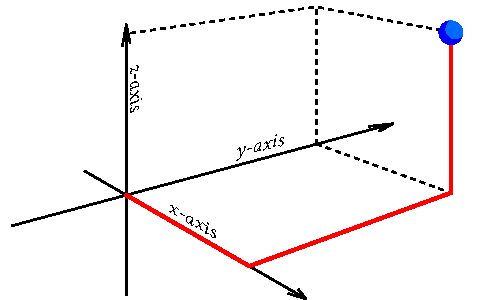
\includegraphics{01xyz-axes.pdf}
  \caption{To determine the location of points in three dimensional
    space (such as the center of the blue sphere in this drawing), we
    should choose three coordinate axes, and specify three numbers:
    the $x$, $y$, and $z$ coordinates of the point.  }
\end{figure}




\section{Geometric description of vectors} %{{{1
\label{sec:geometric-description-of-vectors}
A vector is an arrow connecting two points.  If the points are $A$ and
$B$ then we call the vector $\tpv AB$. If we translate a vector $\tpv
AB$ \emph{without turning it} then we say that the resulting vector
$\tpv CD$ is the same vector as the original vector $\tpv AB$.  We say
that the arrows $\tpv AB$ and $\tpv PQ$ \emph{both represent the same
  vector.}
\begin{figure}[h]\centering
  \input ../figures/234/005equalvectors.tex
  \caption{$\tpv AB$ and $\tpv CD$ represent the same vector}
\end{figure}
Since both $\tpv AB$ and $\tpv PQ$ are the same vector we will often
want to use a notation for vectors that does not emphasize any
particular choice of initial-~and endpoint.  The notation we will use
in this course is
\[
\va = \tpv AB = \tpv PQ,
\]
i.e., a single letter with an arrow on top will always stand for a
vector in this course.

\begin{figure}[h]\centering
  \def\figfont{\sffamily\footnotesize\color{darkbluegreen}\centering}
  \def\addingvectorsCapA{\parbox{1in}{\figfont%
      to add\\
      two vectors\dots}} \def\addingvectorsCapB{\parbox{1in}{\figfont%
      \dots move one vector until its initial point\dots}}
  \def\addingvectorsCapC{\parbox{1in}{\figfont%
      \dots is the end point of the other\dots} }
  \def\addingvectorsCapD{\parbox{1in}{\figfont%
      \dots and combine them.} } \input
  ../figures/234/005adding-vectors2.pdf_tex
  \caption{Adding vectors}
\end{figure}
\section{Arithmetic of vectors} %{{{1
\label{sec:arithmetic-of-vectors}
To add two vectors $\tpv AB$ and $\tpv PQ$ we first translate the
vector $\tpv PQ$ so that its initial point becomes $B$; let the result
of this translation be the vector $\tpv BC$.  Then, by definition, the
sum of $\tpv AB$ and $\tpv PQ$ is $\tpv AC$: in a formula,
\[
\tpv AB + \tpv PQ = \tpv AB + \tpv BC = \tpv AC.
\]
An equivalent way of adding two vectors $\tpv AB$ and $\tpv PQ$ is to
move the vectors around until they have the same initial point.  Two
vectors with a common initial point form two sides of a parallelogram
(see Figure~\ref{fig:adding-vectors-parallelogram}) and the sum of the
two vectors is the diagonal of that parallelogram.
\begin{figure}[h]
  \input ../figures/234/005adding-vectors-parallelogram.pdf_tex
  \caption{{\bfseries Using a parallelogram to add vectors. } To find
    $\tpv AB + \tpv AD$ we move the vector $\tpv AD$ so that its
    initial point is at $B$, i.e.~the endpoint of $\tpv AB$.  This
    gives us a parallelogram $ABCD$, where $\tpv AD = \tpv BC$.
    Therefore $\tpv AB+\tpv AD = \tpv AB+\tpv BC = \tpv AC$ }
  \label{fig:adding-vectors-parallelogram}
\end{figure}

One can also multiply vectors with numbers.  To multiply a vector
$\va$ with a positive real number $t>0$, we multiply the length of the
vector by a factor $t$, without changing the direction of the vector.
\begin{figure}[h]
  \input ../figures/222/05scalar-mult.pdf_tex
  \caption{Multiplying and subtracting vectors}
\end{figure}
\section{Vector algebra} %{{{1
The addition and multiplication of vectors and numbers satisfy a number of
algebraic properties that should look familiar, as they are very similar to the usual
algebraic properties for adding and multiplying numbers.  Here they are:
\begin{align*}
  \va+\vb&=\vb+\va &&& \text{commutative law}\\
  (\va+\vb)+\vc &= \va+(\vb+\vc) & t\cdot(s\cdot\va) &= (ts)\cdot \va
  &\text{associative laws}\\
  t\cdot(\va+\vb) & = t\va+t\vb & (t+s)\va &= t\va + s\va
  &\text{distributive laws}
\end{align*}
\section{Component representation of vectors} %{{{1
There is a way to represent a vector by specifying a list of numbers instead of by
giving a geometric description of the vector.  To do this for vectors in the plane,
we must first choose a point in the plane, which we will call the origin, and we must
also choose two coordinate axes (the ``$x$'' and ``$y$'' axes).  Once we have made
these choices, we define
\begin{align*}
  \ves1 &= \text{ vector with length $1$, in the direction of the $x$ axis} \\
  \ves2 &= \text{ vector with length $1$, in the direction of the $y$ axis}
\end{align*}
Then any other vector can be written as the sum of a multiple of $\ves1$ and another
multiple of $\ves2$:
\begin{equation}
  \va = a_1\ves1 + a_2 \ves2.
  \label{eq:vector-a-in-components}
\end{equation}
See Figure~\ref{fig:vector-in-components}.
The numbers $a_1$ and $a_2$ are called the \emph{components of the vector $\va$.}  If
we know the components $a_1$ and $a_2$ of a vector, and if we know the two vectors
$\ves1$ and $\ves2$, then we can reconstruct the vector $\va$ by using the formula
\eqref{eq:vector-a-in-components}.

\begin{figure}[h]
  \input{../figures/234/005vector-components.pdf_tex}
  \caption{Describing a vector in terms of its components.}
  \label{fig:vector-in-components}
\end{figure}

\noindent%
Instead of using the notation \eqref{eq:vector-a-in-components}, one very often
writes
\begin{equation}
  \va = \vek a_1 \\ a_2 \tor,
  \text{ or }
  \va = \begin{bmatrix}
    a_1 \\ a_2
  \end{bmatrix}, \text{ or } \va = \langle a_1, a_2\rangle.
  \label{eq:vector-a-as-column-vector}
\end{equation}
This notation says that $\va$ is the vector whose components are $a_1$ and $a_2$; it
can only be used if it is clear how the coordinate axes were chosen.

The first two ways of writing the vector, in which the components
$a_1$ and $a_2$ are listed in a column, is the standard way of writing
``column vectors,'' and is used in linear algebra courses (math 320,
340, 341, etc.), and by most computational software (Matlab$^{\rm
  TM}$, Octave, etc.).  The third way of writing the components also
gets used, especially when one has to type the equations rather than
write them by hand.

The preceding also applies to vectors in three dimensional space:
\begin{figure}[h]\sffamily\color{darkbluegreen}
  \input{../figures/234/005vector-components3D.pdf_tex}
\end{figure}

\section{The dot product} %{{{1
There are two different descriptions of the dot product of two
vectors: one geometric, and the other in terms of the components of
the vectors.

\subsection{Geometric description of the dot product}
If $\va$ and $\vb$ are two given vectors, then, by definition,
\marginpar{\footnotesize\sffamily\centering\color{darkbluegreen}%
  \input ../figures/234/005dot-product.pdf_tex

  The dot product between two vectors.
}
\begin{equation}
  \label{eq:dotproduct-geometric}
  \va\dpp\vb = \|\va\| \, \|\vb\|\,\cos \theta,
\end{equation}
where $\theta$ is the angle between the two vectors $\va$ and $\vb$.

\subsection{The dot product in terms of vector components}
If we choose an orthonormal set of vectors $\ves1,\ves2,\ves3$, and write
\[
  \va = a_1\ves1+a_2\ves2+a_3\ves3=\vek a_1 \\ a_2 \\ a_3 \tor,\qquad
  \vb = b_1\ves1+b_2\ves2+b_3\ves3=\vek b_1 \\ b_2 \\ b_3 \tor,
\]
then
\begin{equation}
  \label{eq:dotproduct-algebraic}
  \va\dpp\vb = a_1b_1 + a_2b_2 + a_3b_3.
\end{equation}
The fact that \eqref{eq:dotproduct-geometric} and \eqref{eq:dotproduct-algebraic}
always give the same result is not obvious (the formulas look very different), and
requires a proof.  A very common proof relies on the law of cosines (it was given in
math 222 -- see also Problem~\ref{prb:law-of-cosines-and-dotprod})

\subsection{Algebraic properties of the dot product}
\label{sec:dotproduct-algebraic-properties}%
The dot product has the following algebraic properties, which we will
use very often throughout this course:
\begin{align*}
  \va\dpp\vb &= \vb\dpp\va & \text{commutative} \\
  s(\va\dpp\vb) &= (s\va)\dpp\vb & \text{associative} \\
  (\va+\vb)\dpp\vc & = \va\dpp\vc + \vb\dpp\vc. & \text{distributive}
\end{align*}
We will not prove these properties here.  Proofs can be given if one
starts either from the algebraic description of the dot-product
\eqref{eq:dotproduct-algebraic}, or from the geometric description
\eqref{eq:dotproduct-geometric} (although the distributive property is
more difficult to prove from the geometric description than from the
algebraic description.)

The sign of the dot product tells us if the angle between two vectors is acute,
obtuse, or if the vectors are perpendicular:
\begin{subequations}
  \begin{align}
    \va\perp\vb  &\iff \va\dpp\vb=0 \\
    \va\dpp\vb>0 &\iff \theta<\frac{\pi}{2}\\
    \va\dpp\vb<0 &\iff \theta>\frac{\pi}{2}.
  \end{align}
\end{subequations}

\section{The cross product} %{{{1
As with the dot product, the cross product of two vectors also has a
geometric description, and a description in terms of components.

\subsection{Geometric description of the cross product} Let $\va$
and $\vb$ be two vectors in three dimensional space, then their
\emph{cross product} is the vector $\va\cp\vb$ that satisfies
\begin{itemize}
\item $\va\cp\vb$ is perpendicular to $\va$, and also to $\vb$
\item the length of $\va\cp\vb$ is given by
  \[
  \|\va\cp\vb\| = \|\va\|\,\|\vb\|\,\sin\theta,
  \]
  where $\theta$ is the angle between the vectors $\va$ and $\vb$,
\item the three vectors $\va$, $\vb$, $\va\cp\vb$ satisfy the
  \emph{right hand rule:} if on your right hand $\va$ is the index
  finger and $\vb$ is the middle finger, then your thumb points in the
  direction of $\va\cp\vb$.  See Figure~\ref{fig:cross-product}.
\end{itemize}
\begin{figure}[t]
  \input ../figures/222/05crossprod-corkscrew.pdf_tex
  \caption{The cross product: $\va\cp\vb$ is perpendicular to both
    $\va$ and $\vb$; its direction follows from the right-hand rule. }
  \label{fig:cross-product}
\end{figure}
The length of the cross product of two vectors has a geometric
interpretation.  Namely, the quantity $\|\va\|\,\|\vb\|\,\sin\theta$
is exactly the are of the parallelogram spanned by the vectors $\va$
and $\vb$.
\begin{figure}[h]
  \input
  ../figures/222/05area-parallelogram-spanned-by-vectors.pdf_tex
\end{figure}

\subsection{Algebraic description of the cross product} If $\va$
and $\vb $ are given by \eqref{eq:dotproduct-geometric}, i.e.~by
\[
\va = a_1\ves1+a_2\ves2+a_3\ves3=\tvek a_1 \\ a_2 \\ a_3 \ttor,\qquad
\vb = b_1\ves1+b_2\ves2+b_3\ves3=\tvek b_1 \\ b_2 \\ b_3 \ttor,
\]
then
\[
\va \cp\vb = \vek
a_2b_3 - a_3b_2\\
a_3b_1 - a_1b_3\\
a_1b_2 - a_2b_3 \tor.
\]

\subsection{Algebraic properties of the cross product}
The cross product has the distributive property, namely,
\begin{equation}
  (\va+\vb)\cp\vc  = \va\cp\vc + \vb\cp\vc,
  \label{eq:cross-product-distributive}
\end{equation}
holds true for any three vectors $\va$, $\vb$, $\vc$.

The cross product is \emph{not commutative}: $\va\cp\vb$ and
$\vb\cp\va$ are not the same thing.  Instead, we have :
\begin{equation}
  \va\cp\vb = -\vb\cp\va.
\end{equation}
Because of this property the cross product is said to be
``\textit{anti-commutative.}''

The associative property fails completely for the cross product: for
most vectors $\va$, $\vb$, $\vc$ one has
\begin{equation}\color{red}
  \carefulnow\carefulnow\qquad
  (\va\cp\vb)\cp\vc\; {\boldsymbol \neq}\; \va\cp(\vb\cp\vc)
  \qquad \carefulnow\carefulnow
  \label{eq:cross-product-not-associative}
\end{equation}

If you need a vector that is perpendicular to two given vectors, take
their cross product.

The length of the cross product $\va\cp\vb$ is the area of the
parallelogram spanned by those vectors.

\section{The triple product} %{{{1
\label{sec:determ-triple-prod}
Just as two vectors in the plane form a parallelogram, three vectors
in space will form a shape called a parallelepiped.  By definition, a
parallelepiped is a solid body each of whose faces is a parallelogram.

\begin{figure}[h]
  \def\svgwidth{200pt}
  \input ../figures/234/01parallelepiped.pdf_tex\hfill
  \def\svgwidth{130pt}
  \input ../figures/234/01parallelepiped-flipped.pdf_tex
  \caption{\textbf{A parallelepiped spanned by three vectors $\va$,
      $\vb$, $\vc$.}  Since the base of the parallelepiped is a
    parallelogram with edges $\vb$ and $\vc$, we have \\
    \null\qquad Area of base~$= \|\vb\cp\vc\|$.\\
    The height of the parallelepiped is $\|\va\|\cos\theta$, and
    therefore the volume is given by \\
    \null\qquad Volume = $\text{height}\cdot\text{area of base}
    = \|\va\| \, \|\vb\cp\vc\| \cos\theta
    = \va\dpp\bigl(\vb\cp\vc\bigr)$.\\
    This derivation applies to the situation on the left, where the
    vector $\va$ and the cross product $\vb\cp\vc$ point in the same
    direction.  If these vectors form an obtuse angle, as is the case
    on the right, then $\cos\theta<0$, and the height is
    $-\|\va\|\cos\theta$.  In that case one has\\
    \null\qquad Volume = $\text{height}\cdot\text{area of base}
    = - \|\va\| \, \|\vb\cp\vc\| \cos\theta 
    = - \va\dpp\bigl(\vb\cp\vc\bigr)$.
  }
  \label{fig:volume-of-parallelpiped}
\end{figure}
If we are given three vectors $\va$, $\vb$, and $\vc$, then the volume
of the parallelepiped they determine is given by the formula
\[
\text{``Volume equals Area of base times height''}
\]
In terms of the three vectors this is
\begin{equation}
  V = \left| \va\dpp\bigl(\vb\cp\vc\bigr)\right|.
  \label{eq:volume-of-parallelpiped}
\end{equation}
A derivation is sketched in Figure~\ref{fig:volume-of-parallelpiped}.
The quantity $\va\dpp(\vb\cp\vc)$ (without the absolute values) is
called the \emph{triple product} of the three vectors $\va$, $\vb$,
and $\vc$.  Apart from its use in computing the volume of a
parallelepiped, the triple product appears in many other contexts.  At
first sight the expression $\va\dpp(\vb\cp\vc)$ suggests that the
order in which the vectors appear is important, but this turns out not
to be true.  One has 
\[
\va\dpp\bigl(\vb\cp\vc\bigr) = \vb\dpp\bigl(\vc\cp\va\bigr) =
\vc\dpp\bigl(\va\cp\vb\bigr)
\]
for any $\va,\vb,\vc$.

\section{Determinants} %{{{1
\label{sec:determinants}
For any four numbers $a$, $b$, $c$, $d$, one defines the $2\times2$
determinant to be
\begin{equation}
  \deter a&b \\ c& d
  \minant
  =ad-bc\,.
  \label{eq:determinant-2x2}
\end{equation}
One can also define $3\times3$ determinants.  Namely, for any nine
numbers $a_1, \dots, c_3$ one defines
\begin{equation}
  \deter
      a_1 & b_1 & c_1 \\
      a_2 & b_2 & c_2 \\
      a_3 & b_3 & c_3
  \minant
  =
  a_1b_2c_3 - a_1b_3c_2 - a_2b_1c_3 + a_2b_3c_1 +a_3b_1c_2 - a_3b_2c_1\,.
  \label{eq:triple-product}
\end{equation}
This can be written as
\begin{align}
  \deter
  \color{red}a_1 & b_1 & c_1 \\
  \color{red}a_2 & b_2 & c_2 \\
  \color{red}a_3 & b_3 & c_3
  \minant
  &={\color{red}a_1}\bigl(b_2c_3-b_3c_2\bigr)
  - {\color{red}a_2}\bigl(b_1c_3-b_3c_1\bigr)
  + {\color{red}a_3}\bigl(b_1c_2-b_2c_1\bigr)
  \label{eq:determinant-expanded-along-column}
  \\
  &= {\color{red}a_1} \deter b_2 & c_2 \\ b_3 & c_3 \minant
  - {\color{red}a_2} \deter b_1 & c_1 \\ b_3 & c_3 \minant
  + {\color{red}a_3} \deter b_1 & b_1 \\ b_2 & b_2 \minant
  \notag
\end{align}
where each coefficient in the first row is multiplied with the
$2\times2$ determined that remains after one deletes the row and
column containing the coefficient.

Instead of expanding along the first row one can also expand along the
first column:
\begin{equation}
  \deter
  \color{red}a_1 & \color{red}b_1 & \color{red}c_1 \\
  a_2 & b_2 & c_2 \\
  a_3 & b_3 & c_3
  \minant
  = {\color{red}a_1}\deter b_2 & c_2 \\ b_3 & c_3 \minant
  - {\color{red}b_1}\deter a_2 & c_2 \\ a_3 & c_3 \minant
  + {\color{red}c_1}\deter a_2 & b_2 \\ a_3 & b_3 \minant
  \label{eq:determinant-expanded-along-row}
\end{equation}
Many other mnemonic devices exist to remember how to compute a
$3\times3$ determinant.  A popular trick is ``Sarrus' rule'' (see
Figure~\ref{fig:Sarrus}.)

One can also define larger determinants, i.e.~$4\times4$, $5\times5$,
etc, and generally $n\times n$ determinants.  The theory, which is
beyond the scope of this course, is treated in linear algebra courses
such as Math 320, 340, or 341.

\section{Determinants, the triple product, and the cross product} %{{{1
\label{sec:determ-triple-prod-cross-prod}
If the numbers $a_1, \dots, c_3$ in a determinant happen to be the
components of three vectors $\va$, $\vb$, $\vc$, i.e.~if
\[
\va = \vek a_1\\ a_2 \\a_3\tor, \vb = \vek b_1\\ b_2 \\b_3\tor, \vc =
\vek c_1\\ c_2 \\c_3\tor,
\]
then the corresponding determinant is exactly the triple product:
\begin{equation}
  \left|
    \begin{array}{ccc}
      a_1 & b_1 & c_1 \\
      a_2 & b_2 & c_2 \\
      a_3 & b_3 & c_3
    \end{array}
  \right|= \va\dpp\bigl(\vb\cp\vc\bigr).
\end{equation}%
\begin{figure}[t]
  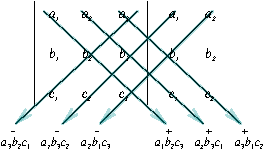
\includegraphics[scale=1.30]{05determinant-shortcut2.pdf}
  \caption{\textbf{Computing $3\times3$ determinants. } There are several
    shortcuts to remember how to compute a $3\times3$ determinant.
    Pictured here is ``Sarrus' rule,'' which tells us to copy the
    first two columns of the determinant to the right of the
    determinant, and read off the six terms in the determinant by
    following the diagonals. }
  \label{fig:Sarrus}
\end{figure}%
Related to this is the following practical trick for computing the
cross product of two column vectors.  Given two column vectors $\vb$
and $\vc$ one can write their cross product as 
\begin{align*}
  \vek b_1\\b_2\\b_3\tor\cp \vek c_1\\c_2\\c_3\tor
  &=
  \deter
  \ves1 & b_1 & c_1 \\
  \ves2 & b_2 & c_2 \\
  \ves3 & b_3 & c_3
  \minant \\
  &=  \deter b_2 & c_2 \\ b_3 & c_3 \minant \ves1
    - \deter b_1 & c_1 \\ b_3 & c_3 \minant \ves2
    + \deter b_1 & b_1 \\ b_2 & b_2 \minant \ves3 .
\end{align*}
The $3\times3$ determinant in this equation is unusual in that some of
its entries are vectors instead of numbers.  The intention of this
notation is that one expand the determinant along the first column, as
in \eqref{eq:determinant-expanded-along-column} and then interpret the
result as a vector.

\section{Defining equations for lines and planes} %{{{1
\label{sec:defin-equat-plan}
Let $\ell$ be a line in the plane, and suppose we know one point $A$ on the
line, and that we also have a vector $\vn$ that is perpendicular to the line
(and we exclude $\vn=\vvv0$.) Such a vector is called a \emph{normal vector} to
the line.  Given any other point $X$ in the plane we can form the vector $\tpv
AX$ and consider its dot-product with the normal.  We have
\[
  \vn \dpp \tpv AX = \|\vn\| \, \|\tpv AX\| \cos \theta,
\]
where $\theta$ is the angle between the normal vector $\vn$ and $\tpv AX$.

\begin{figure}[h]
  \hspace{-1em}\input ../figures/222/05distance-to-line.pdf_tex
\end{figure}
The combination $\|\tpv AX\|\cos \theta$ is, up to its sign, the distance from
the line $\ell$ to the point $X$: If $X$ lies on the side of $\ell$ at which the
normal vector points then $\vn\dpp\tpv AX>0$; if $X$ lies on the other side then
$\vn\dpp\tpv AX<0$.  We therefore have the following formula for \textit{the
distance between a point $X$ and the line $\ell$:}
\begin{equation}
  d = \frac{\vn \dpp \tpv AX	}{\|\vn\|}
  \label{eq:distance-to-line}
\end{equation}
When we use this equation to compute the distance from $X$ to $\ell$, it is good
to recall that if $\vx=\tvek x_1\\x_2\ttor$ and $\va = \tvek a_1\\ a_2\ttor$ are
the position vectors of the points $X$ and $A$, then  
\[
  \tpv AX = \vx-\va = \vek x_1-a_1 \\ x_2-a_2\tor.
\]
Moreover, the length of the normal vector is $\|\vn\| = \sqrt{n_1^2+n_2^2}$, so
we can rewrite \eqref{eq:distance-to-line} as 
\[
  d = \frac{n_1(x_1-a_1) + n_2(x_2-a_2)}{\sqrt{n_1^2 + n_2^2}}.
\]
This last formula is more impressive than \eqref{eq:distance-to-line}, but it is
better to remember \eqref{eq:distance-to-line}.

The equation for the distance from any point $X$ to a given line $\ell$ is also
important because it gives us \emph{the defining equation} for the line $\ell$.
The defining equation is an equation that tells us for any given point $X$ in
the plane if that point is on the line or not.  Since $X$ is on $\ell$ exactly
when the distance from $\ell$ to $X$ vanishes, it follows from
\eqref{eq:distance-to-line} that $X$ is on $\ell$ if and only if 
\begin{equation}
  \vn\dpp\tpv AX = 0.
  \label{eq:defining-eqn-for-line}
\end{equation}
We can again rewrite this equation in a few different ways.  If we want to write
it in terms of the position vectors of $A$ and $X$, then we get
\[
  \vn \dpp \bigl(\vx-\va\bigr) = 0, \qquad
  \text{ i.e.: }\qquad
  \vn\dpp\vx = \vn\dpp\va.
\]
Written without vectors, but in terms of the coordinates of the points $A$,
$X$, and the components of the normal vector $\vn$, we can write this last
version of our equation as
\[
  n_1x_1+n_2x_2 = n_1a_1+n_2a_2.
\]


\section{Problems} %{{{1
\problemfont
\begin{multicols}{2}
\problem Draw two vectors $\va$ and $\vb$ for which %{{{2
$\va$ has length 3, $\vb$ has length $5$, and for which $\va\dpp\vb=-12$.

How many solutions are there?%
\answer %{{{2
The problem is open-ended because it doesn't specify what ``draw'' means.

If you are allowed to use a calculator and a protractor, then you could use the
dot product to compute the angle $\theta$ between the two vectors, then, using
your protractor, draw two line segments that make this angle, and mark off
lengths 3 and 7 to get the vectors.  From the dot-product and the two lengths
you find $3\times5\times\cos\theta = -12$, so $\cos\theta = - \frac{12}{15}=
-0.8$, which implies $\theta = \arccos (-0.8) \approx 2.498\dots$ radians, or
$\theta\approx 143.13\dots$ degrees.

Or, you could assume $\va=3\ves1$, which has length 3, and $\vb=\tvek
b_1\\b_2\ttor$.  The condition that $\vb$ have length 5 then says
$b_1^2 + b_2^2 = 5^2 = 25$, while the dot-product is $\va\dpp\vb = a_1b_1+a_2b_2
= 3b_1$.  Since the dot-product must be $-12$ we find $b_1=-\frac{12}{3}=-4$.
Using the length of $\vb$ leads to $b_2=\sqrt{25-(-4)^2} = \pm3$.  Thus we find
two solutions: $\vb = \tvek 4\\ \pm3\ttor = 4\ves1\pm\ves3$.

You make the drawing.
\endanswer

\problem %{{{2  given vectors a, c, find vector b so that a x b = c
You could say this problem is about ``cross division,'' i.e.~can you solve
$\va\cp\vb=\vc$ for $\vb$ if you know $\va$ and $\vc$?

\subprob Let %{{{3
\begin{gather*}
  \va =\ves1-\ves3,\\
  \vc = \ves1+3\ves2+2\ves3.
\end{gather*}
Find a vector $\vb$ for which $\va\cp\vb=\vc$, if there is such a thing.  (Hint:
if $\vc=\va\cp\vb$, then what do you know about $\va\dpp\vc$?)
\answer%{{{3
$\va\dpp\vc=\va\dpp(\va\cp\vb) =0$, but for the two given vectors i the problem
$\va\dpp\vc = -1\neq0$, so there cannot be a vector $\vb$ with $\va\cp\vb=\vc$.
\endanswer

\subprob Let $\va = 2\ves1-\ves3$, and $\vc = \ves1+3\ves2+2\ves3$.%{{{3
Find a vector $\vb$ for which $\va\cp\vb=\vc$, if such a thing exists. %
\answer
In this case $\va\perp\vc$, so the argument from the first part of this problem
doesn't rule out that there might be a solution.  So let's try $\vb =
\tvek b_1\\b_2\\b_3\ttor$.  Then
\[
  \va\cp\vb
  = \vek b_2 \\ -b_1-2b_3 \\ 2b_2\tor \stackrel?= \vc
  = \vek 1\\3\\2\tor.
\]
Solving this for $b_1$, $b_2$, and $b_3$ leads to $b_2=1$, and $-b_1-2b_3=3$ as
only remaining equation.  Since we have found $b_2$ there are still two unknowns
left.  We can choose an arbitrary $b_3$ and set $b_1 = -3-2b_3$, e.g.~$b_3=0$
works, provided we choose $b_1 = -3$.
\endanswer

\problem Which of the following vector equations are true for any pair %{{{2
of vectors $\va$ and $\vb$?  Either give a proof (using the algebraic
properties or the algebraic or geometric descriptions).

\subprob $(\va+\vb)\dpp(\va-\vb) = \|\va\|^2 - \|\vb\|^2$~?

~\hfill%
\answer%{{{2
True:
\begin{align*}
  (\va+\vb)\dpp(\va-\vb) &=(\va+\vb) \dpp \va  - (\va+\vb) \dpp\vb\\
  &= \va \dpp \va +\vb \dpp \va  - \va \dpp\vb - \vb \dpp\vb\\
  &= \|\va\|^2 + \| \vb \|^2.
\end{align*}
\endanswer

\subprob  If  $\va\perp\vb$ then\\[1ex]
\null\quad$\|\va+\vb\|^2 = \|\va\|^2 + \|\vb\|^2$~?%
\answer%{{{2
True:  This is Pythagoras' theorem.  Here is an algebraic derivation:
\begin{align*}
  \|\va+\vb\|^2 &= (\va+\vb) \dpp (\va+\vb)\\
  &= (\va+\vb) \dpp \va  + (\va+\vb) \dpp\vb\\
  &= \va \dpp \va +\vb \dpp \va  + \va \dpp\vb + \vb \dpp\vb\\
  &= \|\va\|^2 + 2 \va \dpp\vb + \| \vb \|^2\\
  &= \|\va\|^2 + \| \vb \|^2.
\end{align*}
\endanswer

\subprob If  $\va\perp\vb$ then\\[1ex]
\null\quad$ \|\va-\vb\|^2 = \|\va\|^2 - \|\vb\|^2$  ~?%
\answer%{{{2
Not so.
The same computation as for the previous problem shows
\begin{align*}
  \|\va - \vb\|^2 &= (\va-\vb) \dpp (\va-\vb)\\
  &= (\va-\vb) \dpp \va  - (\va-\vb) \dpp\vb\\
  &= \va \dpp \va -\vb \dpp \va  - \va \dpp\vb + \vb \dpp\vb\\
  &= \|\va\|^2 - 2 \va \dpp\vb + \| \vb \|^2\\
  &= \|\va\|^2 + \| \vb \|^2.
\end{align*}
Therefore
\[
\|\va-\vb\|^2 = \|\va\|^2 - \|\vb\|^2
\]
only is true if $\vb=\vvv0$.
\endanswer

%%\problem ``Cramer's rule.''  Suppose we have to find solutions $x$,%{{{2
%%$y$, $z$, of the following linear equations:
%%\begin{align*}
%%  a_1x+b_1y+c_1z & = d_1 \\
%%  a_2x+b_2y+c_2z & = d_2 \\
%%  a_3x+b_3y+c_3z & = d_3
%%\end{align*}
%%
%%\subprob Show that you can write these equations as
%%\[
%%x\va + y\vb + z\vc = \vd
%%\]
%%for certain vectors $\va$, $\vb$, $\vc$, and $\vd$.
%%
%%\subprob Show how you can get a formula for $x$ by taking the dot
%%product of both sides in the equation $x\va + y\vb + z\vc = \vd$ with
%%the vector $\vb\cp\vc$.
%%
%%\subprob How would you get a similar formula for $y$?  Or $z$?

\problem \label{prb:law-of-cosines-and-dotprod}%{{{2
The \textit{law of cosines} says that in a triangle $\triangle ABC$
for which you know the sides $AB$ and $AC$, as well as the angle
$\angle A$, the length of the opposing side $BC$ is given by
\begin{multline*}
  (BC)^2 = (AB)^2 + (AC)^2\\  - 2(AB)(AC)\cos\angle A.
\end{multline*}
Show how you can use the dot product to (re)prove this law.

Hint: consider the vector equation $\tpv BC = \tpv AC - \tpv AB$.  You will need both
the geometric description \eqref{eq:dotproduct-geometric} of the dot product, and the
algebraic properties from \S~\ref{sec:dotproduct-algebraic-properties}.

\problem True or False:%{{{2

\subprob If $\va\perp\vb$ and also $\vb\perp\vc$\\[0.5ex]
  \null\hfill then $\va\perp\vc$ ?

\subprob If $\va\perp\vb$ and also $\va\perp\vc$\\[0.5ex]
  \null\hfill then $\va\perp(\vb+\vc)$ ?

\subprob If $\va\perp\vb$ and also $\vb\perp\vc$\\[0.5ex]
  \null\hfill  then $\vb\perp(\va-\vc)$ ?

\subprob If $\va\perp\vb+\vc$ and also $\va\perp\vb-\vc$\\[0.5ex]
  \null\hfill  then $\va\perp\vb$ ?

\problem Simplify the following expressions%{{{2

\subprob \(  (\va+\vb)\cp(\va+\vb) \)
\answer%{{{2
\(  (\va+\vb)\cp(\va+\vb) =\vvv0 \)
\endanswer
%
\subprob \(  (\va+\vb+\vc)\cp(\va+\vb+\vc) \)
\answer%{{{2
\(  (\va+\vb+\vc)\cp(\va+\vb+\vc) =\vvv0 \)
\endanswer
%
\subprob \(  (\va+\vb+\vc)\cp(\va+\vb+\vc) \)
\answer%{{{2
\(  (\va+\vb+\vc)\cp(\va+\vb+\vc) =\vvv0 \)
\endanswer
%
\subprob $(\va+\vb-\vc) \cp (\va-\vb+\vc)$

\subprob $(\va+\vb-\vc) \dpp (\va-\vb+\vc)$
\end{multicols}
\noproblemfont

\chapter{Parametric curves and vector functions} %{{{1

\subsection{Vector functions} %{{{2
So far in calculus we have only considered functions $y=f(x)$ where both the
independent variable $x$ and the dependent variable $y$ are real numbers.

A \emph{vector function} is a function of one variable whose values are vectors
instead of numbers.  One way to specify a vector function is to say what its
components are:
\[
  \vx(t) = \vek x(t) \\ y(t) \\ z(t)\tor = x(t)\ves1 +y(t)\ves2 + z(t)\ves3.
\]
\subsection*{Example} For instance,
\[
  \vx(\theta) = \vek\cos \theta \\ 0 \\\theta\tor  = \cos\theta\,\ves1 + \theta\,\ves3
\]
defines a vector function.  Here we have called the independent variable $\theta$
instead of $t$.

\subsection{The derivative of a vector function} %{{{2
If $\vx(t)$ is a vector function, then we can define its derivative in
the same way as we did for ordinary functions. Namely, we set
\[
\vx'(t) \stackrel{\rm def}= \lim_{\Delta t\to0} \frac{\vx(t+\Delta t)
  - \vx(t)}{\Delta t}.
\]
For this to make sense we would have to define what the limit of a
vector function is.  This can be done, but will not go into the
precise definitions in this course.  More important for our use is
that if the components of a vector function $\vx(t)$ are given, then
the derivative can be computed by just differentiating those
components:
\begin{equation}
  \vx'(t) = \vek
  x'(t) \\ y'(t) \\z'(t)
  \tor.
  \label{eq:derivative-of-vector-function}
\end{equation}
\subsection*{Example} For instance, the derivative of the vector
function from the previous example is
\[
\frac{d\vx}{d\theta} = \frac{d}{d\theta}\vek\cos \theta \\ 0
\\\theta\tor = \vek - \sin\theta \\ 0 \\ 1 \tor = -\sin\theta\,\ves1 +
\ves3.
\]

\subsection{Using vector functions to describe motion} %{{{2
We could describe the motion of a point $P$ in the plane by specifying
the $x$ and $y$ coordinates $x=x(t)$, $y=y(t)$ of the point at any
time $t$.  If the point is moving in three dimensional space then we
would also specify its $z$ coordinate $z=z(t)$.  The curve that is
traced out by the point $P$ is called a \emph{parametrized curve,} or
a \emph{parametric curve.}  The quantity $t$ is called the
\emph{parameter.}

\subsection{Lines}
Consider the motion given by
\begin{equation}
  \vx(t) = \va + t\vv
  \label{eq:straight-line-constant-velocity}
\end{equation}
where $\va $ and $\vv$ are given constant vectors.
\begin{figure}[h]
  \centering
  \input ../figures/234/005linear-motion.pdf_tex
  \caption{\textbf{Vector form of linear motion given by $\vx(t) = \va+t\vv$. } To
  see what this motion looks like, draw $\vx(t)$ for a few different values
  of $t$.  At time $t=0$ we have $\vx(0) = \va$; at time $t=1$ we have $\vx(1) =
  \va+\vv$, so in one time unit our point has moved by the vector $\vv$; another time
  unit later, we have $\vx(2) = \va+2\vv$, so that the point moved again by the
  vector $\vv$. After time $t$ has gone by, the position vector of the point is
  $\vx(t) = \va+t\vv$, so that the point has moved by $t\vv$ since the initial time
  $t=0$.  }
  \label{fig:vector-form-linear-motion}
\end{figure}
We say that $\vx(t)$ given by
\eqref{eq:straight-line-constant-velocity} describes motion with
constant velocity, whose velocity vector is $\vv$.


\subsection{Circular motion}

\subsection{The cycloid}
The \emph{cycloid} is the parametric curve defined by the following vector function
\begin{equation}
  \vx(\theta) = \vek R\theta - R\sin\theta \\ R-R\cos\theta\tor.
  \label{eq:cycloid}
\end{equation}
Here $R>0$ is a constant.
\begin{figure}[h]
  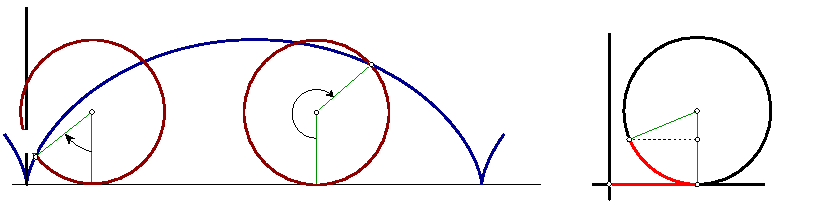
\includegraphics{06cycloid.pdf}
  \caption{\textbf{The cycloid. }  A wheel of radius $R$ rolls over the $x$-axis.
  Initially the wheel touches the $x$-axis at the origin $O$.  The cycloid is the
  curve traced out by a point $X$ on the wheel.}
\end{figure}
\begin{figure}[h]
  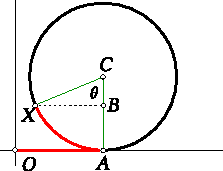
\includegraphics{06cycloid-derivation.pdf}
  \caption{\textbf{Derivation of the cycloid motion. }  The red arc $AX$ and the red
  line segment $OA$ have the same length.  Since $AX$ has length $R\theta$, the $x$
  coordinates of the points $A$, $B$, and $C$ are $R\theta$. The right triangle $CXB$
  has hypotenuse $R$, so the lengths of $XB$ and $CB$ are $R\sin\theta$, and
  $R\cos\theta$, respectively.  Therefore the coordinates of the point $X$ are
  $x=R\theta - R\sin\theta$, and $y=R-R\cos \theta$.}
\end{figure}

\subsection{The helix}
\[
  \vx(t) = \vek \cos t \\ \sin t\\ \tfrac14 t\tor.
\]
\begin{figure}[h]
  \centering
  \input ../figures/234/05helix.tex
  \caption{One full turn of the Helix}
\end{figure}

\subsection{Velocity and acceleration} %{{{2
\label{sec:veloc-accel}
In one variable calculus we learned that the velocity and acceleration
of a moving point are the first and second derivatives of the point's
position, provided the point is moving on a straight line.  It turns
out that velocity and acceleration have a very similar description for
points moving in the plane or in space, provided we use vectors to
describe the motion of the point.  Thus, instead of using the
coordinates $x(t)$, $y(t)$, and $z(t)$ of the point $P$, we will
consider its \emph{position vector.}  By definition, this is the
vector from the origin to the point $P$, and it is given by
\[
\vx(t) = \vek x(t)\\ y(t)\tor, \text{ or }\quad \vx(t) = \vek x(t)\\
y(t) \\ z(t)\tor.
\]
These formulas show us that the position vector contains more or less
the same information as the coordinate functions $x(t)$, $y(t)$, and
$z(t)$; all we have done is to put these coordinate functions together
in a vector.

\begin{figure}[t]
  \centering
  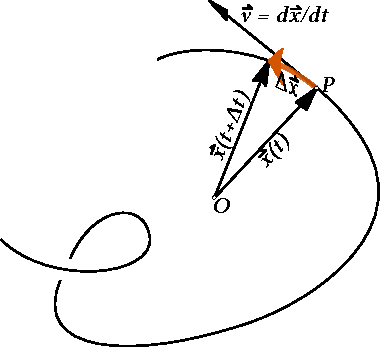
\includegraphics{005velocityistangent.pdf}
  \caption{The parametric curve $\vx(t)$ traces out a curve in space.
    The vector $\vx(t)$ is the position vector of a point $P$ on this
    curve.  As we increase time from $t$ to $ t+\Delta t$, the point
    $P$ moves.  The displacement of the point $P$ is given by
    $\Delta\vx = \vx(t+\Delta t) - \vx(t)$.  The average velocity
    vector during
    this displacement is ``displacement/time'', i.e.\ $\Delta \vx/\Delta t$.\\
    \null\qquad If we let $\Delta t\to 0$, then the average velocity
    becomes the instantaneous velocity at time $t$: $\vv =
    \lim_{\Delta t\to0}\Delta\vx/\Delta t = \vv'(t)$.  This vector is
    tangential to the curve traced out by the vector function
    $\vx(t)$. }
  \label{fig:05velocity-is-deriv-of-position}
\end{figure}
\subsection{Velocity vector of a point moving in space} %{{{2
\label{sec:velocity-of-vector-motion}
let $\vx(t)$ be the position vector of some moving point $P$.  To
define its velocity we go back to the notion that ``velocity'' is
always ``displacement divided by time.''

In this case we consider two instances in time, say, time $t$ and time
$t+ \Delta t$.  Then the position vectors of the point $P$ at these
two different times are $\vx(t)$ and $\vx(t+\Delta t)$.  The
displacement of the point $P$ between these two times is then
\[
\Delta \vx = \vx(t+\Delta t) - \vx(t)
\]
(see Figure~\ref{fig:05velocity-is-deriv-of-position}.)  We say that
the average velocity over the time interval from $t$ to $t+\Delta t$
is ``the displacement divided by $\Delta t$,'' i.e.
\[
\vv_{\rm average} = \frac{\vx(t+\Delta t) - \vx(t)}{\Delta t}.
\]
Note that the average velocity is a vector.  If we write it out in
components, we get a much larger formula:
\[
\vv_{\rm average} = \vek
\dfrac{x(t+\Delta t) - x(t)}{\Delta t} \\[2ex]
\dfrac{y(t+\Delta t) - y(t)}{\Delta t} \\[2ex]
\dfrac{z(t+\Delta t) - z(t)}{\Delta t} \tor.
\]
One big advantage of using vector notation is that many formulas are
much shorter when written in terms of vectors.

To get the instantaneous velocity, we do the same thing as in one
variable calculus: we take the limit as $\Delta t\to0$ of the average
velocity over the time interval from $t$ to $t+\Delta t$.  Thus we get
\begin{equation}
  \vv(t) = \lim_{\Delta t\to0} \frac{\vx(t+\Delta t) - \vx(t)}{\Delta t}
  \stackrel{\rm def}=
  \frac{d\vx}{dt}.
  \label{eq:velocity-of-vector-motion}
\end{equation}
In terms of components this derivative is
\[
\vx'(t)= \frac{d\vx}{dt} = \vek x'(t) \\ y'(t) \\ z'(t) \tor.
\]
Thus to compute the velocity (or derivative) corresponding to any
given vector motion $\vx(t)$ we can simply differentiate each separate
component of $\vx(t)$.

\subsection{Acceleration} %{{{2
The \emph{acceleration vector} is
\[
\va(t)
= \frac{d\vv}{dt}
= \frac{d^2\vx} {dt^2} = \vek x''(t)\\ y''(t) \\ z''(t) \tor.
\]


\subsection{Example--motion on a straight line} %{{{2
Consider the motion given by
\begin{equation}
  \vx(t) = \va + t\vv
  \label{eq:straight-line-constant-velocity}
\end{equation}
where $\va $ and $\vv$ are given constant vectors.  To see what this
motion looks like let's plot a few vectors $\vx(t)$ for different
values of $t$?  At time $t=0$ we have $\vx(0) = \va$; at time $t=1$ we
have $\vx(1) = \va+\vv$, so in one time unit our point has moved by
the vector $\vv$; another time unit later, we have $\vx(2) =
\va+2\vv$, so that the point moved again by the vector $\vv$.
\begin{figure}[h]
  \centering
  \input ../figures/234/005linear-motion.pdf_tex
  \caption{\textbf{Vector form of linear motion: } the initial point
    has positions vector $\va$, }
  \label{fig:vector-form-linear-motion}
\end{figure}
After time $t$ has gone by, the position vector of the point is
$\vx(t) = \va+t\vv$, so that the point has moved by $t\vv$ since the
initial time $t=0$.  We say that $\vx(t)$ given by
\eqref{eq:straight-line-constant-velocity} describes motion with
constant velocity, whose velocity vector is $\vv$.

Here is another reason why we call $\vv$ the velocity vector.  In general the
average velocity of an object over some time interval $t_0<t<t_1$ is the ratio
between ``distance traveled'' and the time that went by.  In the context of a

As the point moves around in the plane or in space, it traces out a curve.  The
velocity vector $\vv(t) = \vx'(t)$ is always tangent to the curve.

The \emph{length} of the curve traced out by $\vx(t), a\le t\le b$ is given by
\[
s = \int_{t=a}^b \|\vx'(t)\|\; dt.
\]


\section{Arc length and the arc length derivative} %{{{1
Recall definition of arc length
\begin{equation}
  \label{eq:arclength-def}
  s = \int \|\vx'(t)\|\; dt.
\end{equation}
and arc length derivative:
\begin{equation}
  \frac{df}{ds} \isdef
  \lim_{\Delta t\to 0}
  \frac{f(t+\Delta t) - f(t)}{s(t+\Delta t) - s(t)}
  \label{eq:arc-length-deriv-def}
\end{equation}
To compute use:
\begin{equation}
  \frac{df}{ds} = \frac{1}{\|\vx'(t)\|} \frac{df(t)}{dt}.
  \label{eq:arclenght-deriv}
\end{equation}
\section{Curvature} %{{{1
\begin{equation}
  \vT = \frac{d\vx}{ds} = \frac{\vx'(t)}{\|\vx'(t)\|}
  \label{eq:unit-tangent-def}
\end{equation}
\begin{equation}
  \frac{d\vT}{ds} = \kappa\; \vN
  \label{eq:first-Serret-Frenet}
\end{equation}
\begin{equation}
  \frac{d\vN}{ds} = -\kappa\vT + \tau\; \vB
  \label{eq:second-Serret-Frenet}
\end{equation}
where
\[
\vB= \vT\cp\vN.
\]
\begin{equation}
  \frac{d\vB}{ds} = -\tau\; \vN
  \label{eq:third-Serret-Frenet}
\end{equation}

\section{Osculating plane} %{{{1

\section{Special cases: 2D} %{{{1
\begin{equation}
  \kappa = \frac{y''}{\bigl(1+(y')^2\bigr)^{3/2}}
  \label{eq:curvature-of-graph}
\end{equation}
\begin{equation}
  \kappa = \frac{d\theta}{ds}
  \label{eq:curvature-is-deriv-of-tangentangle}
\end{equation}
\section{Problems} %{{{1
\problemfont
\problem Suppose a point $P$ is rotating around a line $l$, keeping%{{{2
its distance to the line fixed at $r$, and moving in a plane
perpendicular to the line.  Suppose the point has angular velocity
$\omega$: this means that the angle swept out by the line from $P$ to
$l$ during a time interval of length $t$ is exactly $\omega t$.

In a previous math or physics class it was shown that the velocity of
the point $P$ is $\omega r$, where $r$ is the distance from $P$ to
$l$.

The \emph{angular velocity vector} is defined to be the vector
$\vvv\omega$ whose length is $\omega$, and which is parallel to the
line $l$.  There are two such vectors ($\pm \vvv\omega$).  By
definition $\vvv\omega$ points in the direction in which a corkscrew
would move if it were turning in the same direction as the point $P$.

\begin{figure}[h]
  \begin{center}
    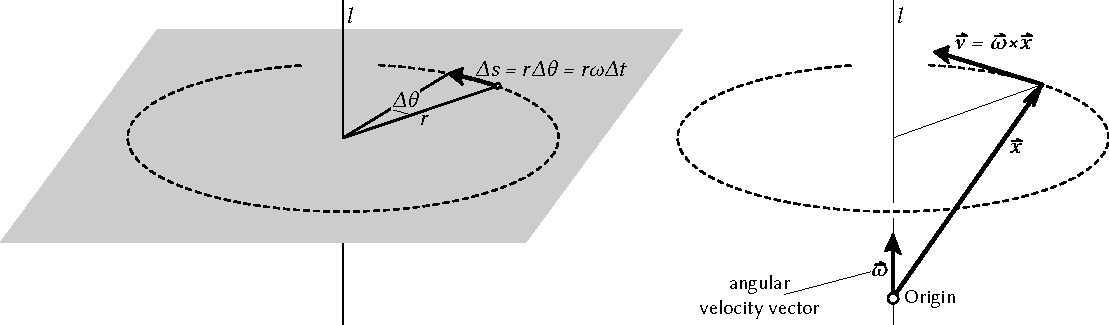
\includegraphics[width=0.9\textwidth]{005angularvelocity.pdf}
  \end{center}
\end{figure}


\subprob Assuming the line $l$ passes through the origin show that the
velocity vector of the point $P$ is $\vv = \vvv\omega \cp \vx$

\subprob Show that the acceleration vector is given by $\va =
\vvv\omega\cp(\vvv\omega\cp\vx)$.

\subprob If someone told you they had computed the acceleration vector
and found $\va =(\vvv\omega\cp\vvv\omega)\cp\vx$, could they be right?
Explain!  What if they told you they got $\va =
\vvv\omega\cp\vvv\omega\cp\vx$?

\subprob True or False (explain your answers):

(a) $\vv\perp \vx$?\qquad (b) $\va\perp \vv$? \qquad (c) $\va$ and
$\vx$ are parallel?

\subprob Include the acceleration vector $\va$ in the above drawing.

\problem Compute the curvature, torsion, tangent, normal and binormal%{{{2
for the following curves

\subprob The parabola: $\vx(t) = \tvek t^2 \\ t\ttor$.  At which point
on the curve is the curvature the largest?

\subprob Neil's parabola: $\tvek t^2\\ t^3\ttor$.  At which point on
the curve is the curvature the largest?

\subprob The helix: $\vx(\theta) =\vek\cos \theta \\ \sin \theta\\
a\theta\tor$ ($a>0$ is a constant).  At which point on the curve is
the curvature the largest?

\problem \subprob Compute the curvature at the point $(x, e^x)$ of the%{{{2
graph of $y=e^x$.
\answer $k(x) = \dfrac{e^x}%{{{2
{\bigl(1+e^{2x}\bigr)^{3/2}}$.
\endanswer

\subprob Which point on the graph of $y=e^x$ has the largest
curvature?
\answer $k'(x) = \dfrac{e^x} {\bigl(1+e^{2x}\bigr)^{5/2}}%{{{2
\bigl(1-2e^{2x}\bigr)$, so the maximal curvature (smallest radius of
curvature) occurs when $x=-\frac{1} {2}\ln{2}$.
\endanswer

\problem \subprob Compute the curvature at the point $(x, \ln x)$ of%{{{2
the graph of $y=\ln x$.

\subprob Which point on the graph of $y=\ln x$ has the largest
curvature?


\problem Show: a curve is plane if and only if its torsion vanishes%{{{2
($\tau = 0$).

\problem Express $\vx'\cp\vx''$ in terms of $\kappa, \tau, \vT, \vN,%{{{2
\vB$ and $\|\vx'\|$.

\problem Let $A(h)$ be the area of the triangle with vertices%{{{2
$\vx(t-h)$, $\vx(t)$ and $\vx(t+h)$.  Compute $\DS \lim_{h\to 0}
\frac{A(h)}{h^3}$.  Hint: use a Taylor expansion $\vx(t+h) = \vx(t) +
h\vx'(t) + \frac{h^2}{2}\vx''(t) + o(h^2)$.

\noproblemfont

\chapter{Functions of more than one variable} %{{{1

\subsection{The graph of a function} %{{{2
In first-year calculus we were concerned with functions of one
variable, meaning the ``input'' is a single real number and the
``output'' is likewise a single real number. At the end of math 222 we
considered functions taking a real number to a vector: for each input
value we get a position in space. Now we turn to functions of several
variables, meaning several input variables, functions.
While we will deal primarily with $n=2$ and to a lesser
extent $n=3$, many of the techniques we discuss can be applied
to larger values of $n$ as well.

\begin{figure}[h]
  \begin{center}
    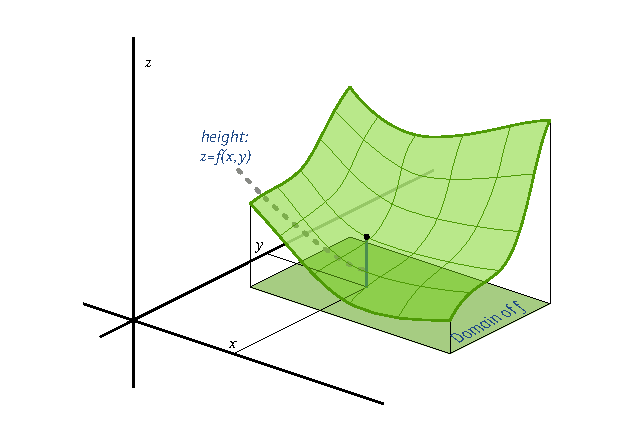
\includegraphics{01Agraph.pdf}
  \end{center}
  \caption{The graph of some function, and its domain (a rectangle in
  this example).}
  \label{fig:01Agraph}
\end{figure}

A function of two variables maps a pair of values $(x,y)$ to a
single real number.  The three-dimensional $xyz$-coordinate system
is a convenient aid in visualizing such functions: above
each point $(x,y)$ in the $xy$-plane we graph the point $(x,y,z)$,
where of course $z=f(x,y)$.

\subsection{Vector notation} We will use vectors all the time in this %{{{2
course.  If $\vx$ is the position vector of the point $(x, y)$ in the
plane, i.e.\ if $\vx = \tvek x\\ y\ttor$, then one writes
\[
f(x, y)  = f(\vx).
\]

\subsection{Example}\label{sec:example-of-a-function1} Consider %{{{2
$f(x,y)=3x+4y-5$. Writing this as $z=3x+4y-5$ and then $3x+4y-z=5$ we
recognize the equation of a plane.  In the form $f(x,y)=3x+4y-5$ the
emphasis has shifted: we now think of $x$ and $y$ as independent
variables and $z$ as a variable dependent on them, but the geometry is
unchanged.

\subsection{Example}\label{sec:example-of-a-function2} You know that %{{{2
$x^2+y^2+z^2=4$ represents a sphere of radius 2. We cannot write this
in the form $z=f(x,y)$, since for each $x$ and $y$ in the disk
$x^2+y^2<4$ there are two corresponding points on the sphere. As with
the equation of a circle, we can resolve this equation into two
functions, $f(x,y)=\sqrt{4-x^2-y^2}$ and $f(x,y)=-\sqrt{4-x^2-y^2}$,
representing the upper and lower hemispheres. Each of these is an
example of a function with a restricted domain: only certain values of
$x$ and $y$ make sense (namely, those for which $x^2+y^2\le 4$) and
the graphs of these functions are limited to a small region of the
plane.


\subsection{Freezing a variable} %{{{2
\begin{multicols}{2}
If a function isn't familiar, then a good strategy for drawing its
graph is to ``\emph{freeze a variable.}'' In other words, to analyze
a function $ z=f(x,y) $ you pretend $ y $ is a constant: then $ x $
is the only independent variable, and you can try to draw the graph
of the function $ z=f(x,y) $, now thinking of this as a function of
only one variable. This graph is a curve in the $ xz $ plane. You
get one such curve for each choice of $ y $. Piecing these graphs
together then gives you the graph of the two-variable function $
z=f(x,y) $.

You could apply the same procedure with the roles of $ x $ and $ y $
switched: i.e. for each fixed $ x $ you try to graph $ z=f(x,y) $ as
a function of the variable $ y $ only, after which you try to fit
all the graphs you get for different values of $ x $ together.

\centerline{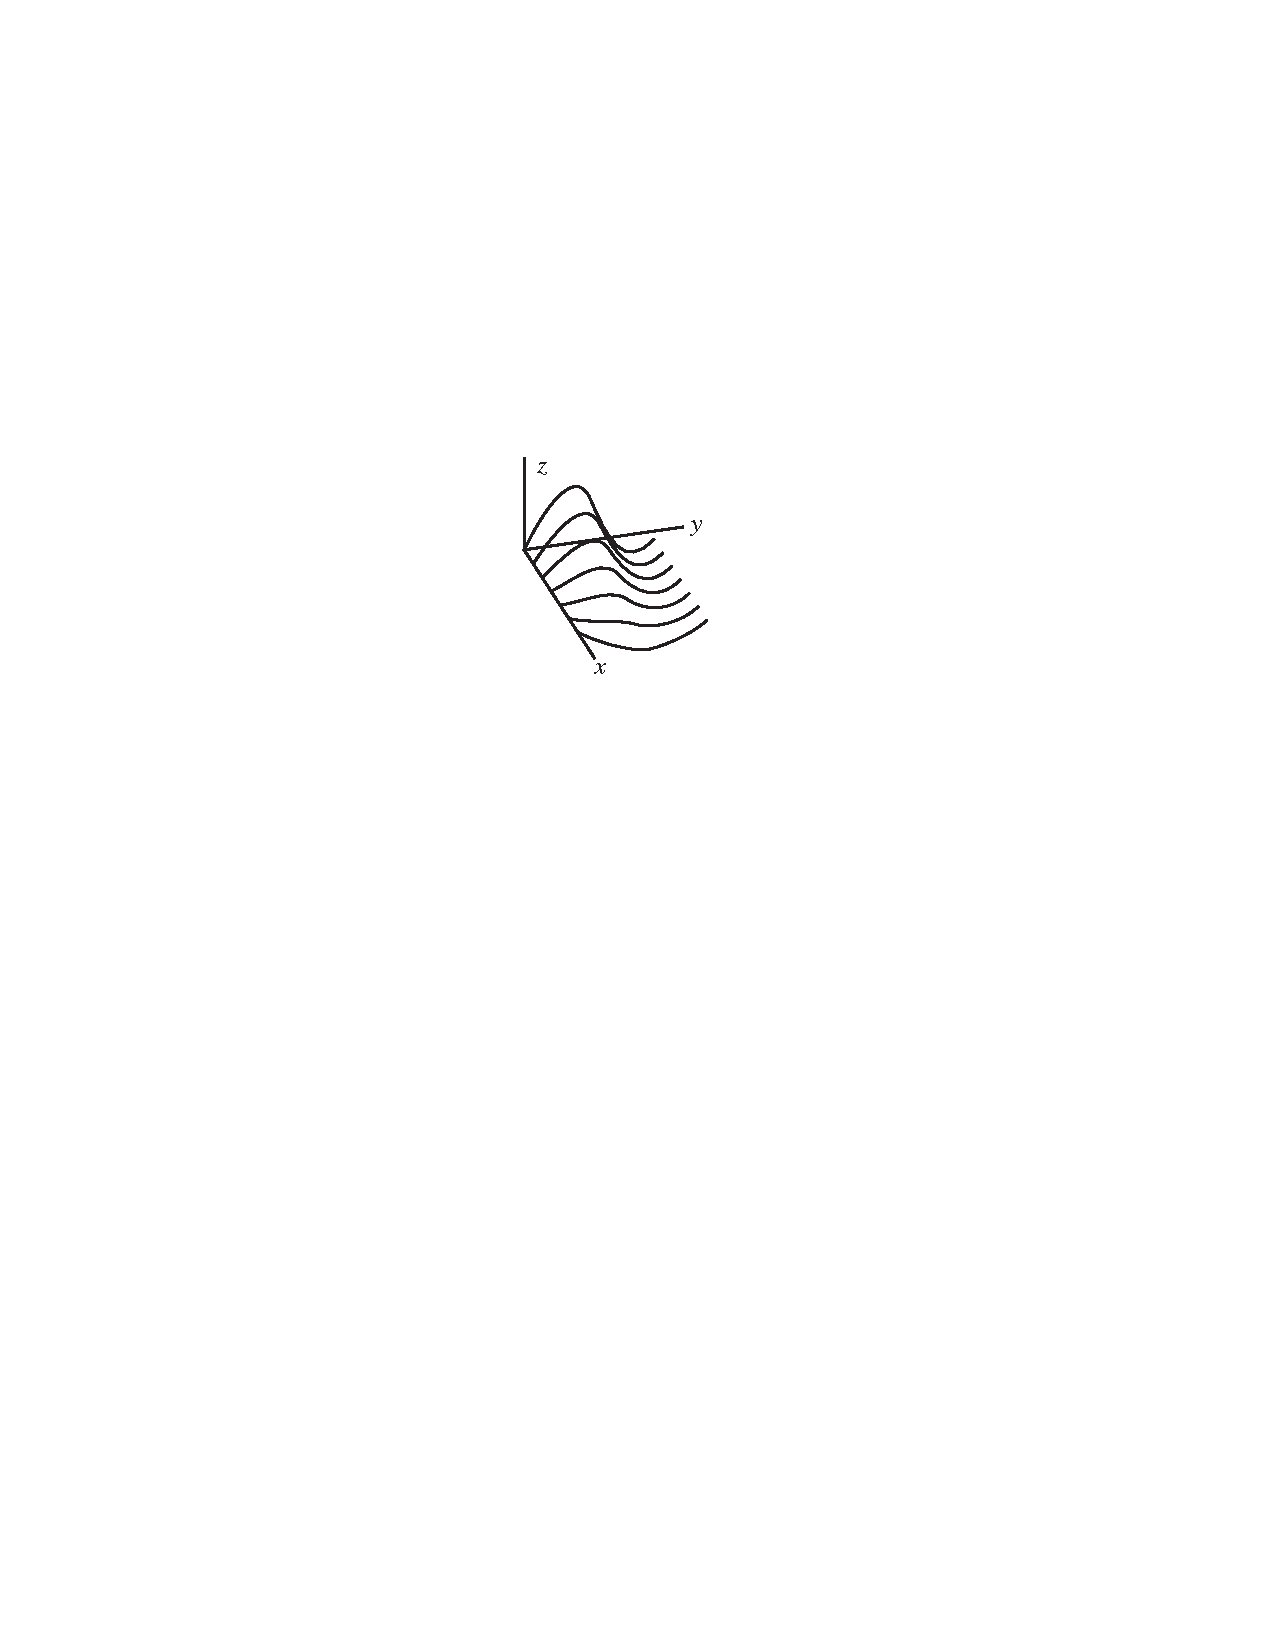
\includegraphics{01frozenvariable.pdf} }
\end{multicols}



\subsection{Example -- draw the graph of $f(x,y) = xy$} %{{{2
\label{sec:example-of-a-function3}
Let's plot the graph of $ z=f(x,y)=xy $.  For each fixed value of $ y $
the graph of $ f(x,y)=xy $ is a straight line with slope $ y $.  For
positive $ y $ the line has positive slope, for negative $ y $ it has
negative slope.   Plotting the graphs of $ z=xy $ for $ y $ frozen at
the values -1,$ -\frac{1}{2} $, $ 0 $, $ \frac{1}{2} $, and 1 gives us
these drawings:

\centerline{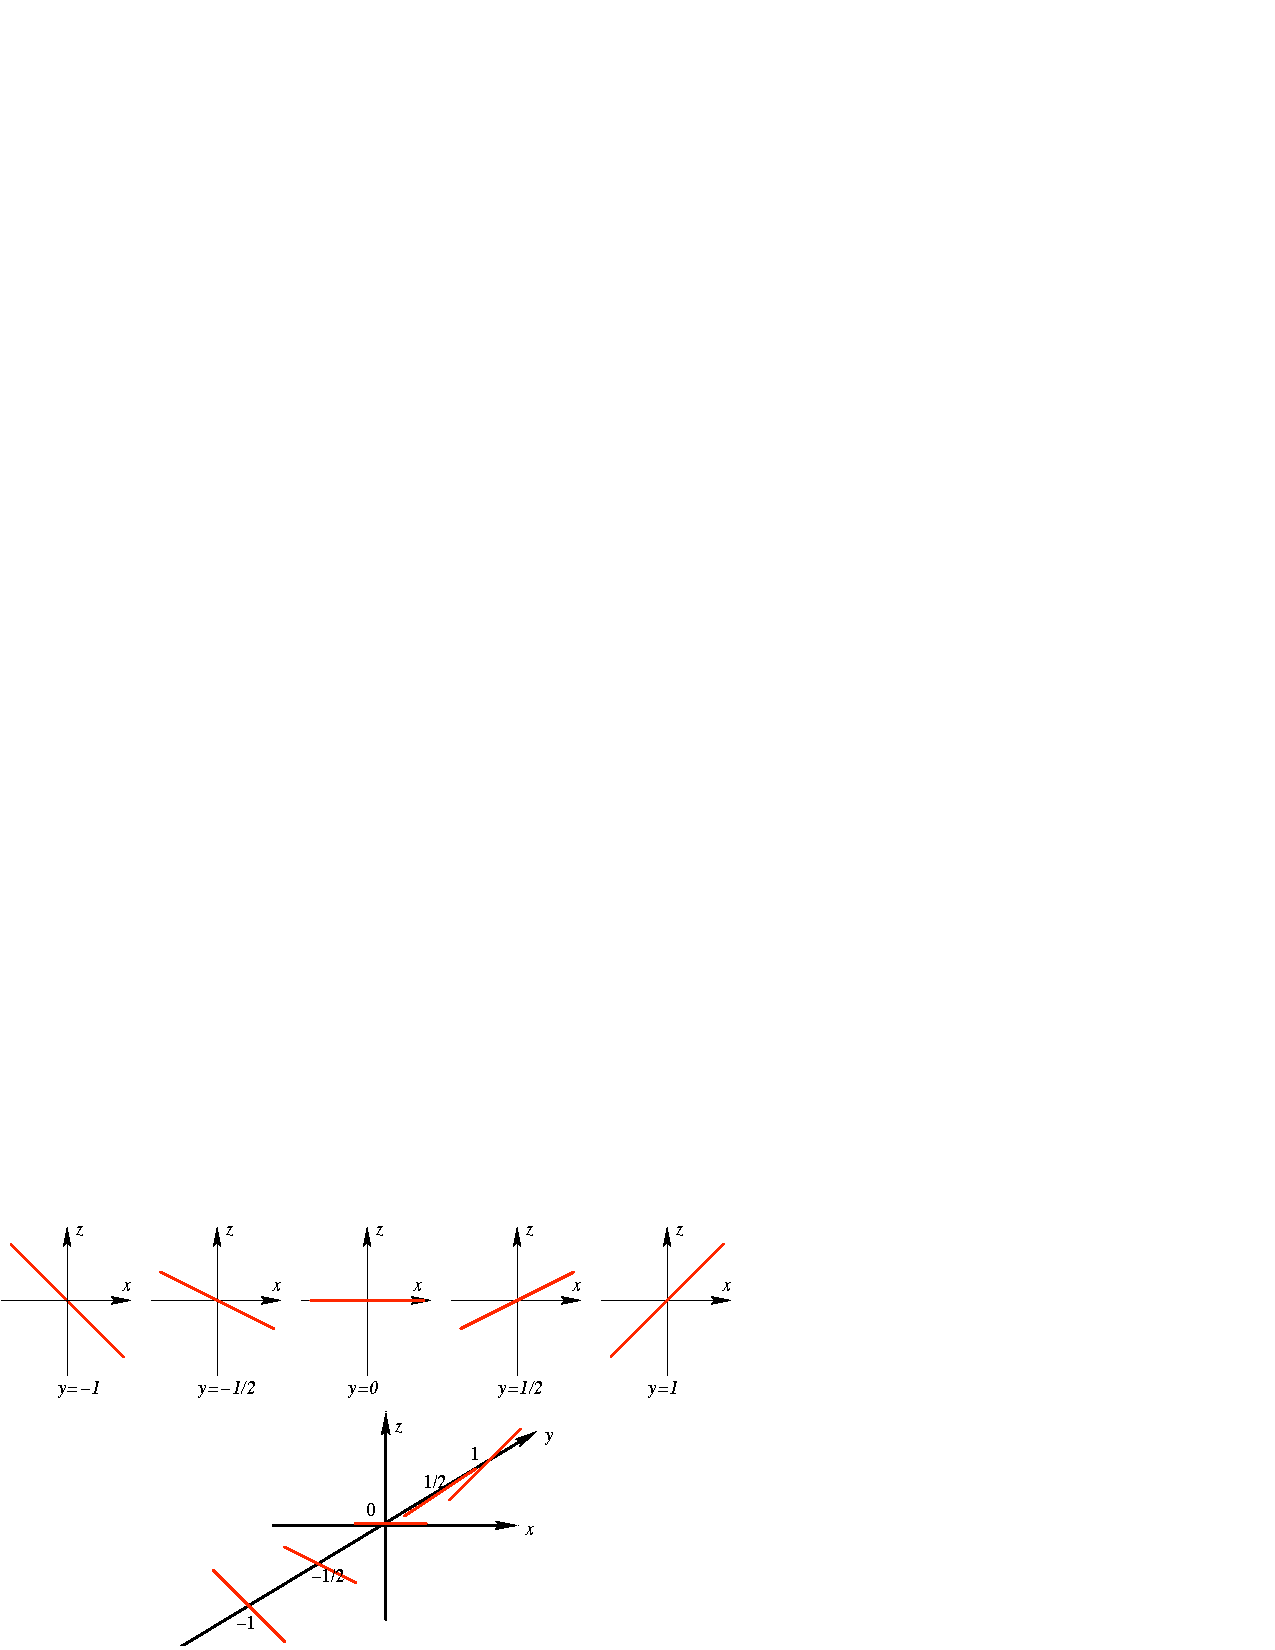
\includegraphics[scale=0.6]{01saddle1.pdf}}


The function $ z=xy $ is symmetric in the $ x $ and $ y $ variables,
so you get similar pictures if you freeze $ x $ and graph $ z=xy $ as
a function of $ y $.  Carefully putting both pictures together gives
something like this:

\centerline{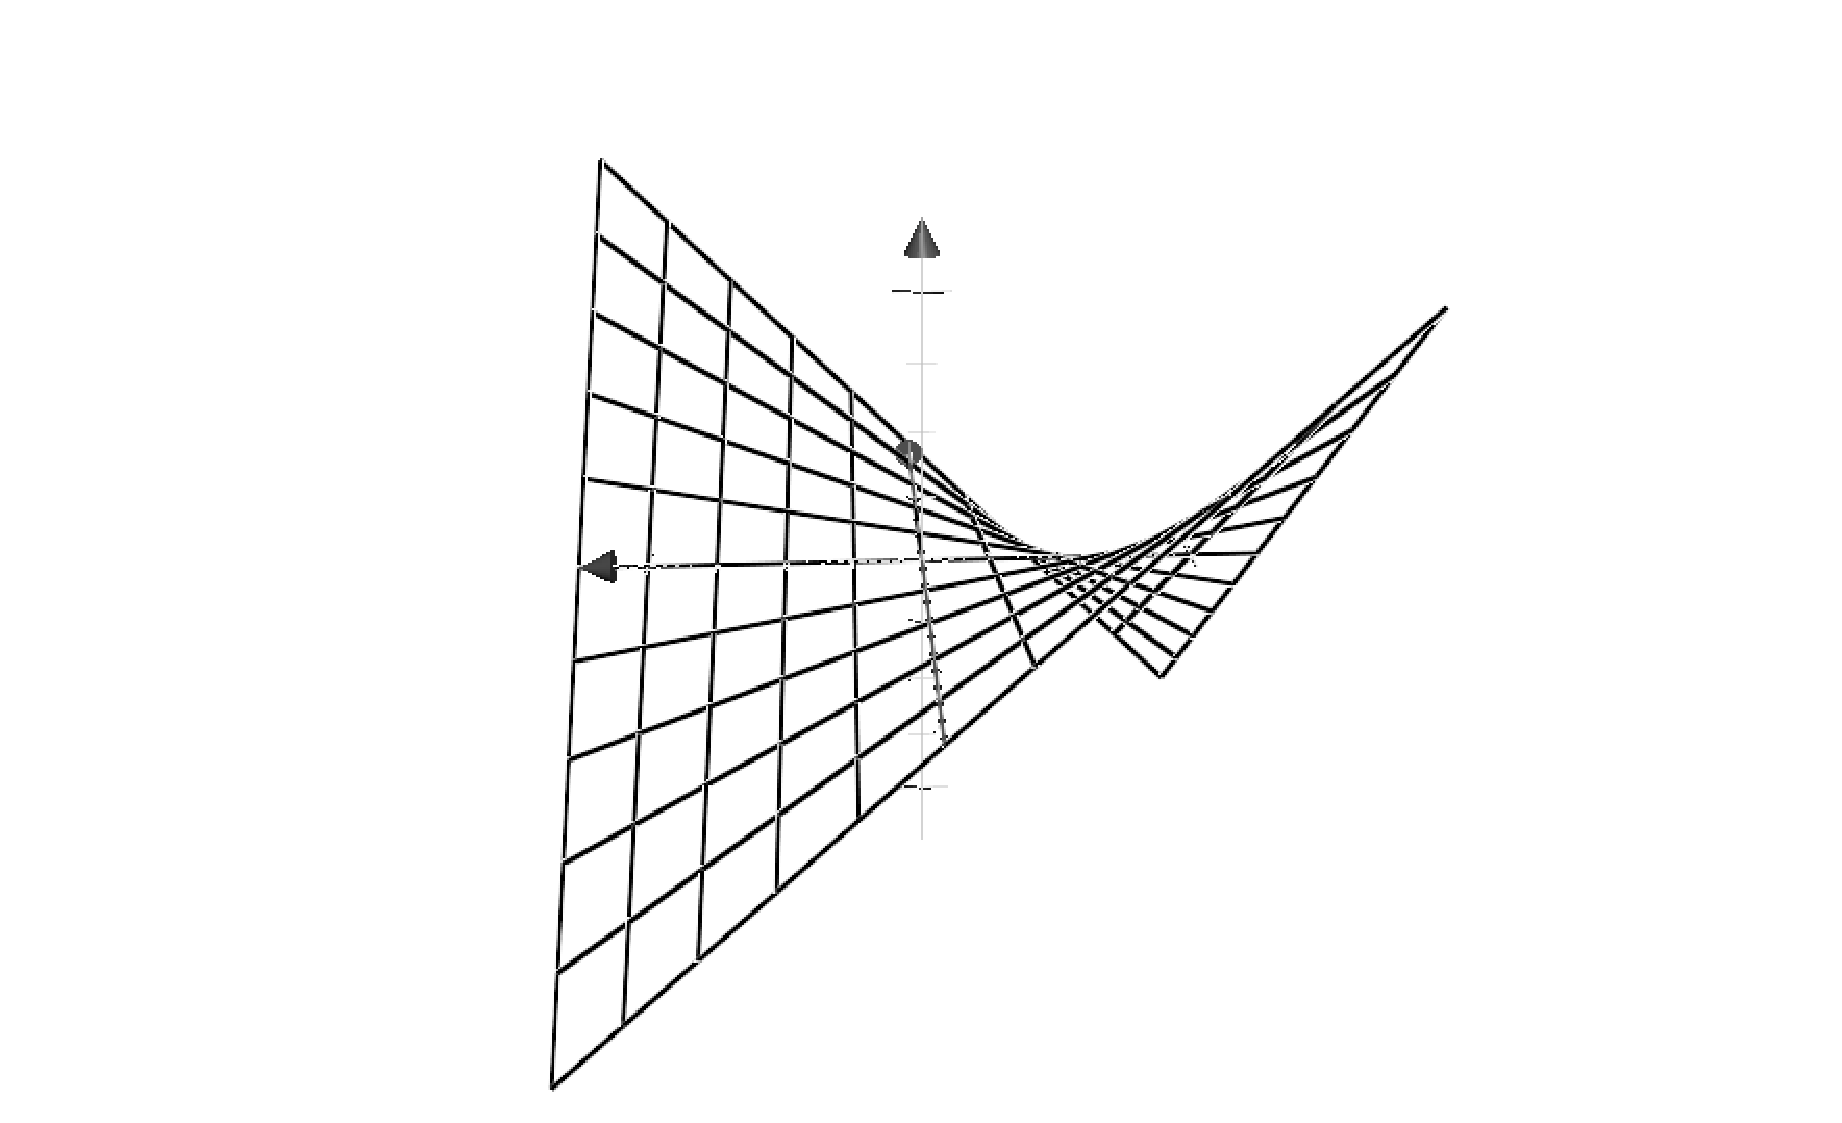
\includegraphics[width=0.3\textwidth]{01saddle3.pdf}}



\subsection{The domain of a function} %{{{2

\begin{multicols}{2}

Just as with functions of one variable, functions of two variables
have a \emph{domain}, consisting of all the points $(x, y)$ in the
plain for which $f(x,y)$ is defined.  For functions of one variable
the domain is usually an interval, but for functions of two
variables the domain can have more interesting shapes.  In the
drawing on the left here, the function $f(x,y)$ is defined to be the
inverse of the distance from the point $(x, y)$ to the curve $E$ in
the picture.  This function is only defined when this distance is
not zero (otherwise you can't divide by the distance\ldots), so the
domain of this function consists of all points which do not lie on
the curve.

\centerline{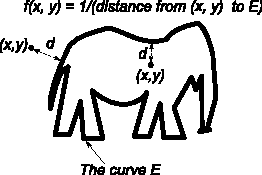
\includegraphics{01elephant.pdf}}
\end{multicols}
\subsection{Example}  What is the domain of the function %{{{2
\[
f(x, y) = \frac{1}{\sqrt{1-x-y}}\quad??
\]
Clearly the function is defined if the quantity under the square root
is nonnegative (otherwise you can't take the square root), and not
zero (otherwise you can't divide by the resulting square root).  So
the domain consists of all points with $1-x-y>0$, or, equivalently,
$y<1-x$.  The domain consists of all points in the plane which line
below the graph of $y=1-x$.



\section{Open and closed sets in $\R^n$} %{{{1
Intervals in the real line come in four kinds, depending on whether
they include their endpoints or not: you can have $(a,b)$, $(a, b]$,
$[a, b)$ and $[a,b]$, and those are all the possibilities.  With
domains in the plane, or in space there are many more possibilities,
and it will sometimes be important to distinguish between domains
which include all their ``endpoints'' and those that don't.  In the
present context one doesn't say ``endpoint'' but speaks of
\emph{boundary point} instead.  To define what a boundary point is, it
turns out that you need to resort to $\varepsilon$ and $\delta$ again,
or a least to $\varepsilon$.
Here is some terminology which we will use:
\begin{itemize}
\item $B_r(p)$ is the ball with center $p$ and radius $r$.

\item $G\subset \R^n$ is \emph{open} if for every point $p$ in $G$ there is an
  $\varepsilon>0$ such that $G$ contains $B_\varepsilon(p)$.

\item $G\subset\R^n$ is \emph{closed} if its complement is open.

\item $p$ is a \emph{boundary point} of $G$ if $B_r(p)$ always contains both
  points from $G$ and from its complement, no matter how small you
  choose $r>0$.
\end{itemize}
The following intuitive description is good enough for math 234: $G$
is closed if it contains all its boundary points; $G$ is open if it
contains none of its boundary points.

\begin{figure}[ht]\centering
  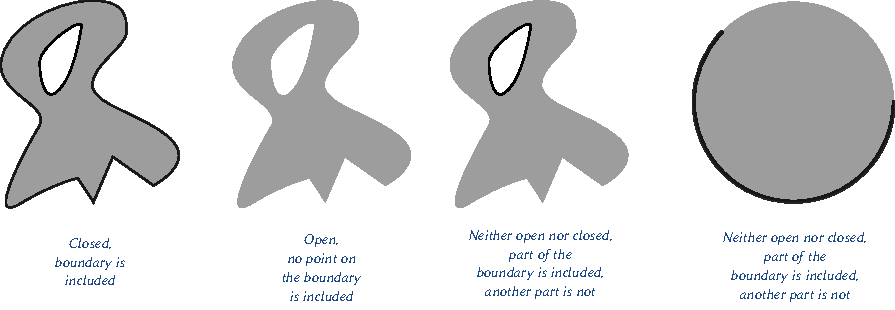
\includegraphics[width=\textwidth]{01openANDclosed.pdf}
  \caption{Some domains in the plane.  Points in the domain are shaded
  gray.  Boundary points which are included in the domain are marked
  in black.}
  \label{fig:01openANDclosed}
\end{figure}

\subsection{Example}\label{sec:openClosedExample} Consider the three domains %{{{2
\begin{align*}
  G_1 &= \text{all points $(x, y)$ with $x^2+y^2<1$}\\
  G_2 &= \text{all points $(x, y)$ with $x^2+y^2\le1$}\\
  G_3 &= \text{all points $(x, y)$ with $-1\leq x\leq 1$ and
  $-\sqrt{1-x^2}<y\leq \sqrt{1-x^2}$}
\end{align*}
For all three domains the boundary points are the points on the unit
circle.  $G_1$ contains none of its boundary points, so it is called
``open'';  $G_2$ contains all its boundary points, so it is called
``closed'';  $G_3$ contains some but not all of its boundary points,
so it is neither open nor closed.



\section{More examples of visualization of Functions} %{{{1

You can visualize a function $f$ of two variables by means of its
graph, but this is not the only way.  There are at least two
alternatives.  The first is in terms of \emph{level sets}, the other
is as a \emph{movie of a graph of a function of one variable}.

\emph{Level sets} are defined as follows.  Given a function $z=f(x,
y)$ and a number $c$, the level set at level $c$ is the set of all
points in the plane which satisfy $f(x, y) = c$; in symbols,
\[
\text{``Level set of $f$ at level $c$''}
\stackrel{\rm def}{=}
\left\{ (x, y) : f(x, y) = c \right\}.
\]
To describe a function in terms of its level sets, one usually picks a
range of values for the constant $c$ and draws the level sets
corresponding to the chosen values of $c$ in one figure.

While the graph is a three-dimensional object, the level set is a set
of points in the plane, usually a curve.  Level sets are therefore
easier to draw than graphs.

\subsection{Example}\label{sec:01levelsetexample} %{{{2
What are the level sets of the function $f(x, y) = 3-x-y$?

For any given number $c$ the level set at level $c$ of $f$ contains
exactly those points $(x, y)$ which satisfy $f(x, y) = c$, i.e.\
$3-x-y = c$.  This is a line, and it is the graph of $y= 3-c-x$:  so
it is the line with slope $-1$ and ``$y$-intercept'' $3-c$.


\subsection{Level sets of the saddle surface}  What are the level sets: %{{{2
of the function whose graph we drew in \S~\ref{sec:example-of-a-function3}?

The function was given by $f(x, y)= xy$, so the level set at level
$c$ consists of all points $(x, y)$ in the plane which satisfy
$xy=c$.  For instance, if $c=1$, then you get the familiar hyperbola
$y=1/x$.  For other positive values of $c$ you get similar hyperbolas,
and for negative $c$ you get hyperbolas in the 2nd and 4th quadrants.

The level at $c=0$ is exceptional because it is not a hyperbola, but
rather consists of two crossing lines.  Namely, $xy=0$ holds when
either $x=0$ or $y=0$ holds, so the level set at $c=0$ is the union of
the $x$-axis and the $y$-axis.

\begin{figure}[htb]
  \begin{center}
    \begin{picture} (240.000000,176.533333)(0,0)
    \put(0.0, 0.0){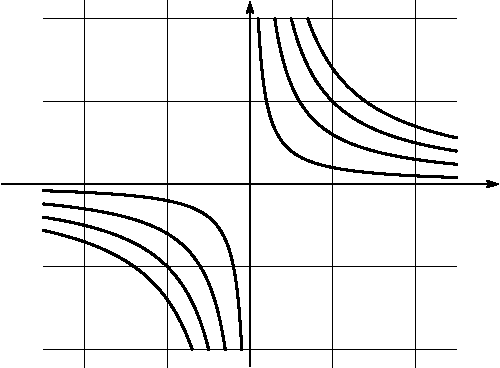
\includegraphics{01saddlelevels.pdf}}
        \put(221.17,  91.44){\sffamily\itshape \makebox[0pt][l]{{\footnotesize \tt$xy=$0.2}}}
    \put( 18.83,  83.09){\sffamily\itshape \makebox[0pt][r]{{\footnotesize \tt$xy=$0.2}}}
    \put(221.17,  97.79){\sffamily\itshape \makebox[0pt][l]{{\footnotesize \tt$xy=$0.6}}}
    \put( 18.83,  76.75){\sffamily\itshape \makebox[0pt][r]{{\footnotesize \tt$xy=$0.6}}}
    \put(221.17, 104.13){\sffamily\itshape \makebox[0pt][l]{{\footnotesize \tt$xy=$1.0}}}
    \put( 18.83,  70.40){\sffamily\itshape \makebox[0pt][r]{{\footnotesize \tt$xy=$1.0}}}
    \put(221.17, 110.48){\sffamily\itshape \makebox[0pt][l]{{\footnotesize \tt$xy=$1.4}}}
    \put( 18.83,  64.05){\sffamily\itshape \makebox[0pt][r]{{\footnotesize \tt$xy=$1.4}}}

\end{picture}

  \end{center}
  \caption{A few level sets of the function $f(x, y) = xy$.  Only
  positive levels are shown.  }
  \label{fig:saddlelevels}
\end{figure}


\subsection{An example from the ``real'' world} %{{{2
\label{sec:01mendotaexample}  Here is a function of local interest.
The domain of the function is the water surface of Lake Mendota (let's
pretend this is a plane domain), and the function, which I'll call $d$
instead of $f$, is given by $d(x, y) = $ the depth of the lake at
location $(x, y)$.  There's no formula for this function, but the
limnology department of the UW has measured the depth and presented
the results in terms of the level sets of the function $d$.


\begin{center}\sffamily
  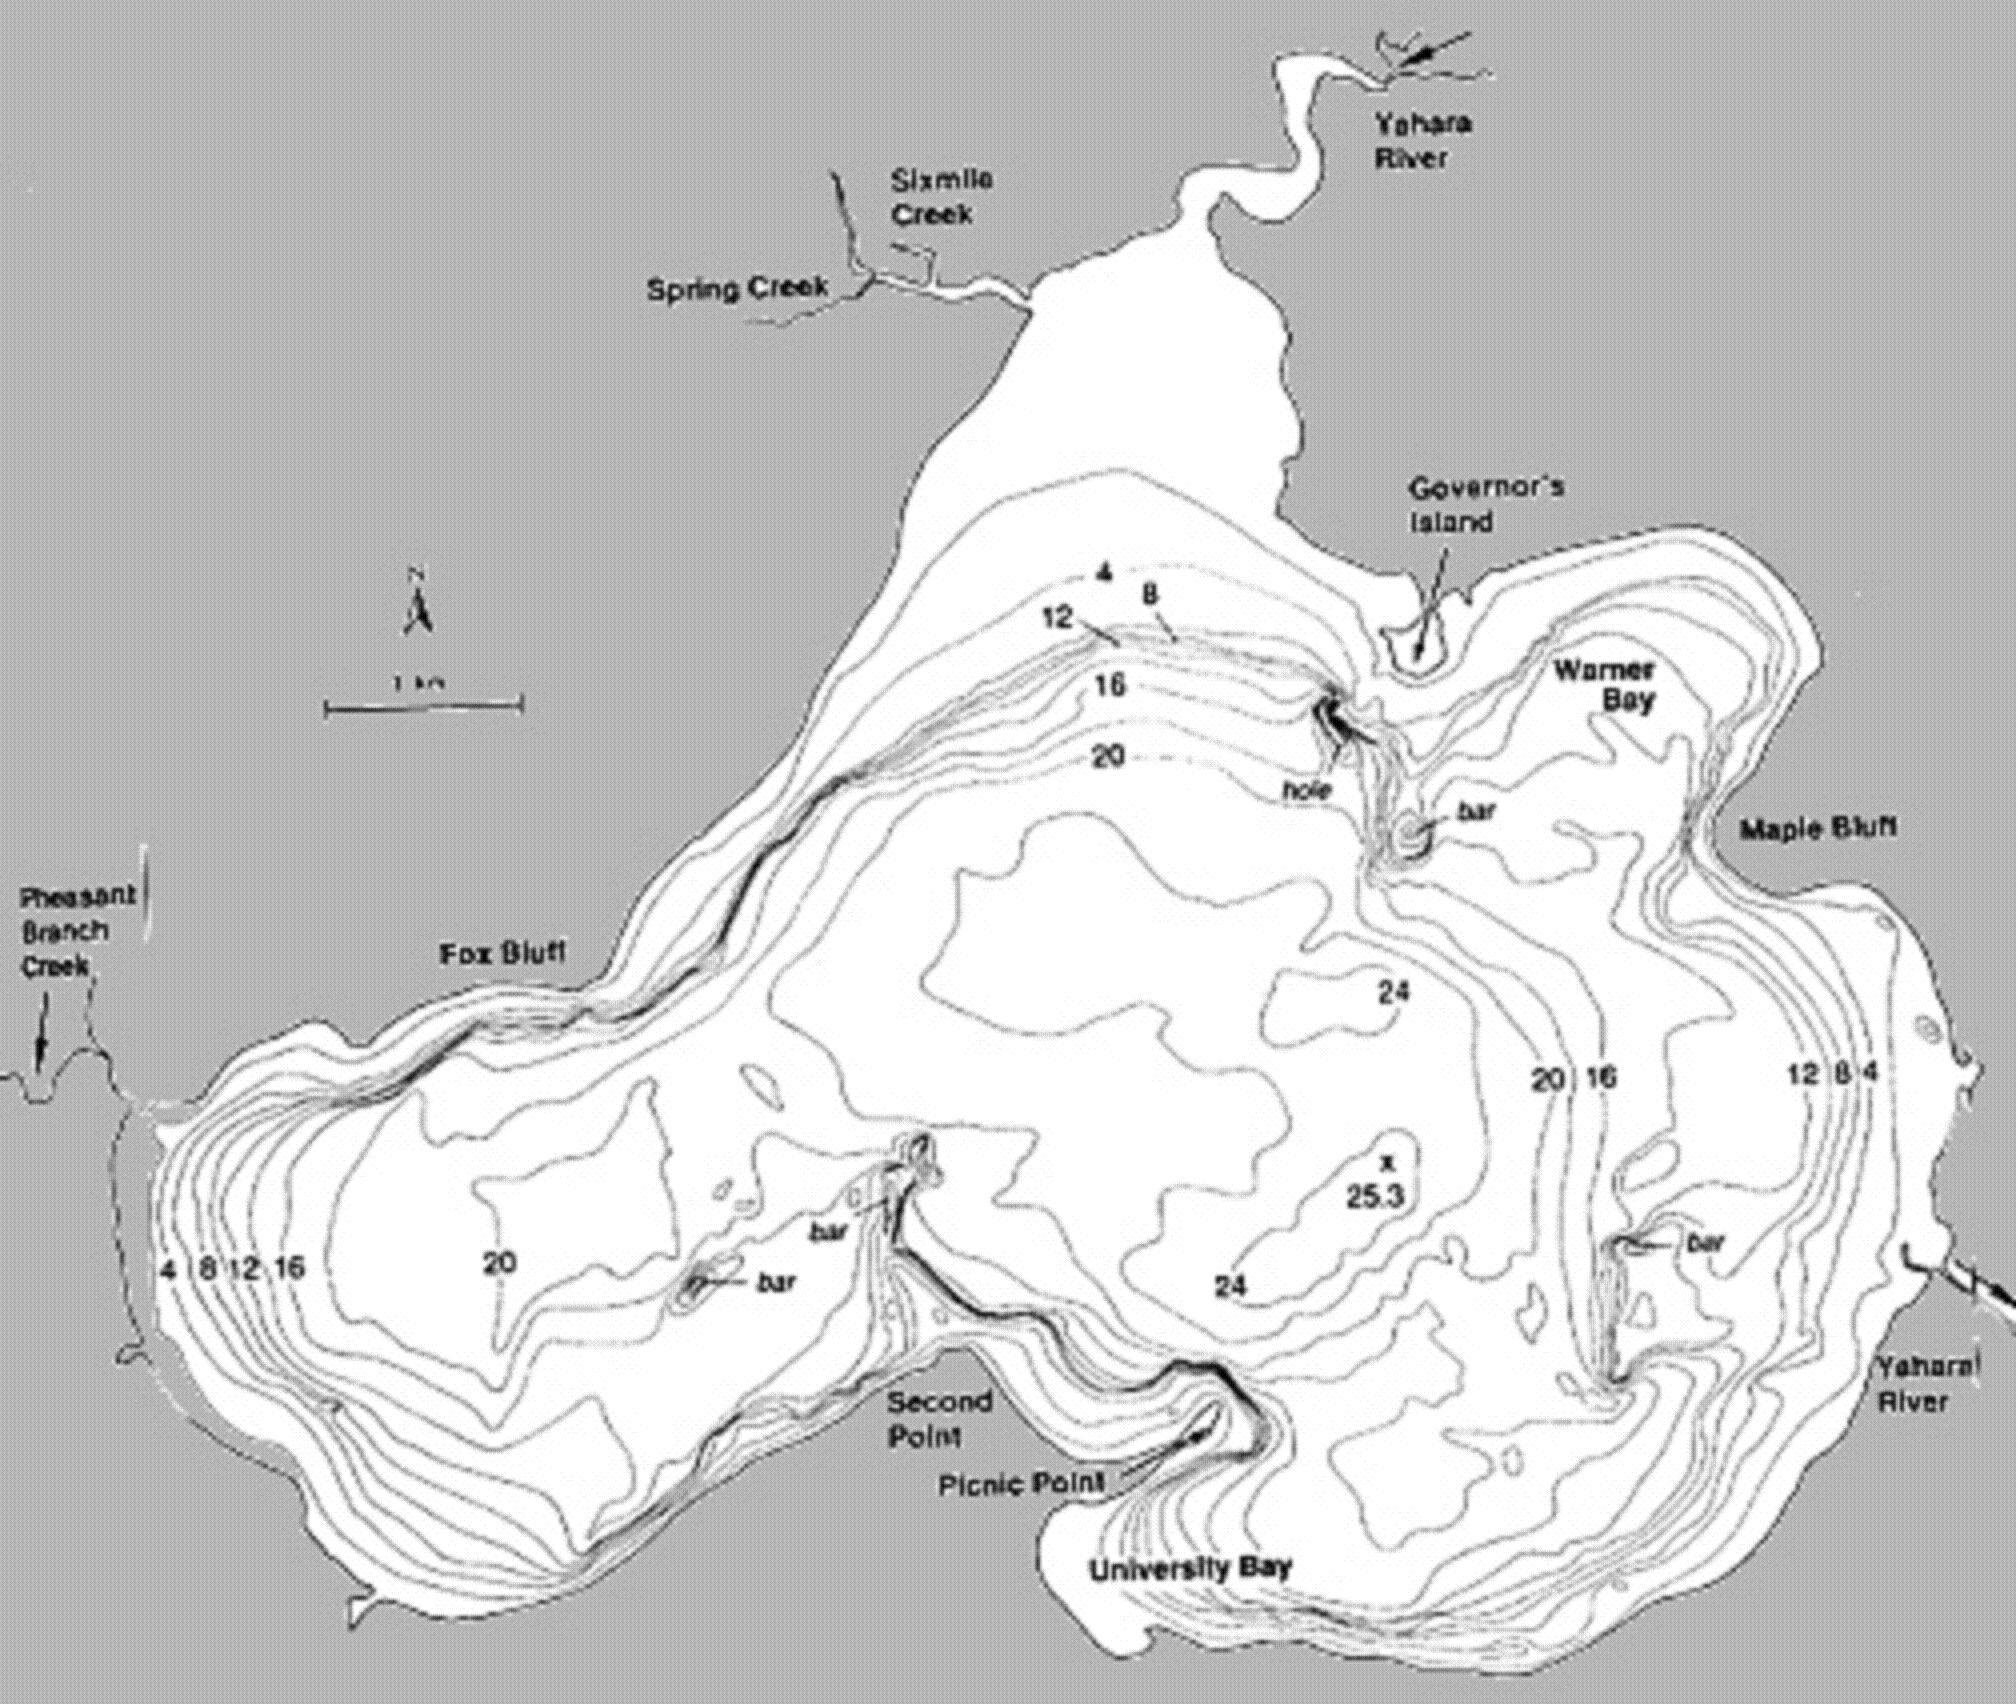
\includegraphics[width=0.75\textwidth]{01Mendota2.jpeg}

  The level curves of a function $z=d(x, y)$.  The domain
  of this function is the lake, \\
  and $d(x, y)$ is the depth in meters of Lake Mendota at $(x, y)$.\\
  See
  \url{http://limnology.wisc.edu/lake_information/mendota/mendota.html}
\end{center}


\subsection{Moving graphs} %{{{2
There's another way of visualizing a function $z=f(x, y)$ of two
variables where you think of one of the independent variables (e.g.\
$y$) as ``time.''  The final picture is not one static picture of a
three dimensional surface, but rather a movie of a graph which is
moving around in the $xz$ plane.

If you have a function $z=f(x, y)$, then let us think of $y$ as time,
and let us relabel it as $t$, so that we are looking at the function
$z=f(x,t)$. Now at each moment in time $t$ we have a function $z=f(x,t)$
of one variable $x$ whose graph you can try to draw. Think of this graph
as a still-image. Then as you let time $t$ vary, putting the still images
in a sequence, you get a movie of a graph of a changing function of one
variable.

For instance, if the function is once again the saddle surface
function $z=xy$, then we would be considering the function $z=xt$. At
each moment $t$ the graph of $z=xt$ is a line with slope $t$. Putting
together these graphs gives a movie of a line which begins with a line
of rather negative slope;  during the movie the slope increases,
and in the middle our line has achieved horizontality;  finally, the
closing shot presents us with a line with a very positive slope.
Here are some stills from the movie:

\begin{center}
  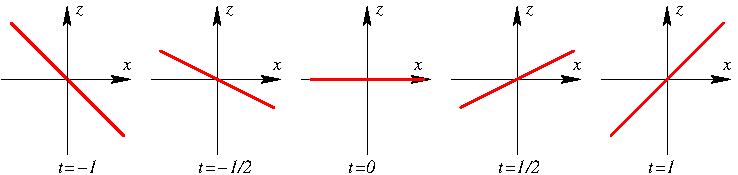
\includegraphics{01saddle-movie.pdf}
\end{center}

So you see that this interpretation is not very different from the
procedure of ``freezing the $y$ variable.'' The only real difference
lies in what you do with all the separate graphs you get after you
freeze a variable. In one case you try to piece them together to make a
bigger drawing of a three-dimensional object, in the other you put them
together to make a motion picture.



\section*{Problems} %{{{1

\problemfont

In the problems in this stage of the course, you will be asked to
``sketch the graph of a function.''  From math 221 you remember that
this meant you had to find minima, maxima, inflection points, and other
features of the graph.  In 234 you will learn to do the same for
functions of two (and more) variables, but for now you should try to
use the method of ``freezing a variable'' or other similar tricks to
get an idea of what the graph of $f$ looks like.

You can use a graphing program (such as \texttt{Grapher.app} on the
Mac, and \texttt{GraphCalc} on Windows) to check your answer.

\begin{center}
  \framebox{\parbox{0.4\textwidth}{Note: very often students try to
      fit their drawings into a region the size of a post-it.  In this
      course, whenever you make a drawing, especially if it's a
      three-dimensional drawing, \emph{make it large!}  Use half a
      page for a drawing.  Make sure you have enough paper, try to
      find lots of cheap scrap paper.}}
\end{center}

\problem  Make careful drawings of the graphs of the three functions%{{{2
in the examples in \S\ref{sec:example-of-a-function1}, and
\S\ref{sec:example-of-a-function2}.


Find the domain of these functions.  Also, label the axes in every drawing
you make.

\problem\label{prb:some-functions}%{{{2
Which functions of two variables $z=f(x, y)$ are defined by the
following formulae?  Find the domain of each function.  Then draw the
domain.  Try to sketch their graphs.

\answer%{{{2
\textbf{You should use a graphing program to produce pictures
of the graphs in these problems.}
\endanswer

\subprob $z-x^2=0$\hspace{7em}
\answer%{{{2
$z-x^2=0$.
Domain $\R^2$.  Graph is a \emph{parabolic cylinder} and consists of
horizontal lines perpendicular to the $xz$-plane, going through the
parabola $y=x^2$ in that plane.

Level sets: parallel straight lines $x=\pm\sqrt{z}$ if $z>0$,
the $x$ axis if $z=0$, the empty set if $z<0$.
\endanswer
\subprob $z^2-x=0$\hspace{7em}
\answer%{{{2
$z^2-x=0$.
Implicit function.
At least two functions are defined, namely $z=\pm \sqrt{x}$.
Domain: all points $(x,y)$ with $x\ge 0$.
Graph is \emph{half a parabolic cylinder} and consists of
horizontal lines perpendicular to the $xz$-plane, going through the
parabola $z=\sqrt x$ (or $z=-\sqrt x$, depending on which function
you choose) in that plane.

Level sets (assuming we choose the function $z=+\sqrt{x}$):
the line $x=z^2$ if $z\ge0$, empty set otherwise.
\endanswer
\subprob $z-x^2-y^2=0$\\
\answer%{{{2
$z-x^2-y^2=0$.
Domain is the whole plane.
Graph is a paraboloid of revolution, obtained by rotating the
parabola $z=x^2$ in the $xz$-plane around the $z$ axis.

Level sets: circle with radius $\sqrt{z}$ for $z>0$,
the origin for $z=0$ (note: this level set is a point rather than a curve),
empty for $z<0$.
\endanswer
\subprob $z^2-x^2-y^2=0$
\answer%{{{2
$z^2-x^2-y^2=0$.
Implicit function.  Domain all of $\R^2$.
Possible functions are $z=\pm\sqrt{x^2+y^2}$.
Graph is the cone obtained by rotating the
half line $z=x, x\geq0$ in the $xz$-plane around the $z$ axis
(or the half line $z=-x, x\geq0$, if you chose $z=-\sqrt{x^2+y^2}$.)

Level sets (assuming we choose $z=+\sqrt{x^2+y^2}$):  circle with radius
$z$ when $z>0$, origin when $z=0$, empty when $z<0$.

\endanswer
\subprob $xyz=1$
\answer%{{{2
$xyz=1$.
Domain the whole plain with the $x$ and $y$-axes removed, i.e.\ all
points $(x, y)$ with $xy\ne0$.
Function is $f(x, y) = \frac{1} {xy}$.
For each $y$ the graph is the hyperbola $z=1/(yx)$ which is just the
standard hyperbola $z=1/x$ stretched vertically by a factor $1/y$.
As $y\to 0$ this factor goes to $\infty$.
\endanswer
\subprob $xy/z^2=1$\\
\answer%{{{2
$xy/z^2=1$.
Implicit function.
Domain first and third quadrants (all points with $xy>0$).
Functions $z= \pm \sqrt{xy}$.
Cross sections with planes $y=$constant are half parabolas.

Note: Harder to see, but the surface with equation $xy=z^2$ is in fact
the cone obtained by rotating the $x$-axis around the line
$x=y$ in the $xy$-plane.
\endanswer
\subprob $x+y+z^2=0$
\subprob $x+y+z^2=1$

\problem Figure \ref{fig:saddlelevels} only presents level sets%{{{2
$f(x, y)=c$ of the function $f(x, y) = xy$ for some \emph{positive} values
of $c$.  What does the zero set look like, and what do the level sets
$f(x, y) = c$ with $c<0$ look like?

\problem
\label{prb:distance-to-square-level-sets}
Let $Q$ be the square in the plane consisting of all points $(x,y)$
with $|x|\le1$, $|y|\le1$.  This problem is about the so-called
\emph{distance function} to $Q$.  This function is defined as
follows:  $f(x, y)$ is the distance from the point $(x,y)$ to the
point in $Q$ nearest to $(x,y)$.

\subprob Which point in $Q$ is nearest to $(0, \frac12)$?  Which is
closest to $(0, 2)$?  Which is closest to $(3,4)$?
\answer%{{{2
$(0, \frac{1} {2})$ is in the square $Q$, so it is the point closest to
$(0, \frac{1} {2})$.\\
The point $(0,1)$ on the top edge of the square is closest to $(0,2)$.\\
The corner point $(1,1)$ is closest to $(3,4)$.
\endanswer

\subprob Compute $f(0, \frac12)$, $f(0,2)$ and $f(3, 4))$.
\answer%{{{2
$f(0, \frac12) =0 $;
$f(0,2)=1$ and $f(3, 4))=\sqrt{2^2+3^2}=\sqrt{13}$.
\endanswer

\subprob What is the zero set of $f$?
\answer%{{{2
The zero set of $f$ is the square $Q$.
\endanswer

\subprob Draw the level sets of $f$ at levels $-1$, 1, 2, and 3.  Describe
the general level set $f(x, y) = c$ where $c$ is an arbitrary number.
\answer%{{{2
The level set at level $-1$ is empty.  The others are ``rounded
rectangles,'' see this drawing, in which the square is grey, the dashed
lines are given by $x=\pm1$ or $y=\pm1$.
\begin{center}
    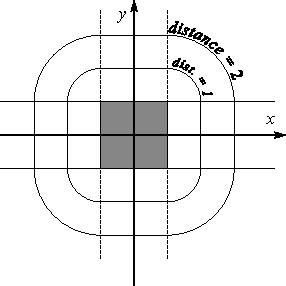
\includegraphics{01distancetosquare.pdf}
\end{center}
\endanswer

\subprob Give a formula for $f(x, y)$.  (It turns out too be hard to
capture the distance function in one formula.  You will have to split the
plane into different regions and describe $f(x,y)$ by different formulas,
according to which region $(x,y)$ belongs to.)
\answer%{{{2
The lines $x=\pm1$ and $y=\pm1$ divide the plane into nine regions.
On each region the function is given by a different formula.
Here they are:
\begin{tabbing}
\=$\boldmath{f(x, y)}$ \=\`\textbf{ if } \ldots \\
\>$0$  \>\` $(x, y)$ in $Q$\\
\>$x-1$ \>\` $x\geq1, |y|\leq 1$\\
\>$y-1$ \>\` $|x|\leq 1, y\geq1$\\
\>$-x-1$ \>\` $x\le-1, |y|\leq 1$\\
\>$-y-1$ \>\` $|x|\leq 1, y\le-1$\\
\>$\sqrt{(x-1)^2+(y-1)^2}$ \>\` $x\ge1$ and $y\ge1$\\
\>$\sqrt{(x-1)^2+(y+1)^2}$ \>\` $x\ge1$ and $y\le-1$\\
\>$\sqrt{(x+1)^2+(y-1)^2}$ \>\` $x\le-1$ and $y\ge1$\\
\>$\sqrt{(x+1)^2+(y+1)^2}$ \>\` $x\le-1$ \& $y\le-1$\\
\end{tabbing}
\endanswer


\problem If $d(x, y)$ is the depth function of Lake Mendota (see%{{{2
\S\ref{sec:01mendotaexample}), then what are the level sets $d(x, y) =
c$ for $c=0$, $c=+10$ and for $c=-10$ (meters)?  What is the level
set $d(x, y) = 400$ (meter)?

\problem For each of the functions in problem \ref{prb:some-functions}%{{{2
draw the level sets at level $z=c$ for a few values of $c$ (as was
done in Figure \ref{fig:saddlelevels} and
\S~\ref{sec:01mendotaexample}).  What does the level set for an
arbitrary $c$ look like?  Are they familiar curves?
\answer%{{{2
See answers to problem \ref{prb:some-functions}.
\endanswer

\problem Describe and explain the relation between the graph of the%{{{2
function $y=g(x)$ of one variable, and the corresponding function
$f(x, y) = g\bigl( \sqrt{x^2+y^2} \bigr)$ of two variables.

What do the level sets of $f(x, y)$ look like?

For instance, if $g(x) = x$, then $f(x, y) = \sqrt{x^2+y^2}$: what is
the relation between the graphs of $g$ and $f$?
\answer%{{{2
The graph of $f$ is obtained by taking the part of the graph of $z=g(x)$
with $x\ge0$ and rotating it around the $z$-axis.

Each level set of $f$ are circles, the origin, or is the empty set.


\endanswer


\problem Find the domain of the following functions of two (or occasionally%{{{2
three) variables:

\subprob  $f(x, y) = \sqrt{9-x^2}+\sqrt{y^2-4}$\hspace{5em}
\answer%{{{2
The two rectangular strips $-3\leq x\leq3, 2\leq y<\infty$ and
$-3\leq x\leq3, -\infty<y\leq-2$.
\endanswer

\subprob  $f(x, y) = \arcsin(x^2+y^2-2)$
\answer%{{{2
By definition $\arcsin(x)$ is only defined if $-1\leq x\leq1$.
For $\arcsin(x^2+y^2-2)$ to be defined, we must therefore have
$-1\leq x^2+y^2-2 \leq 1$, i.e.\ $1\leq x^2+y^2 \leq 3$.

The domain of this function is
the ring-shaped region between the circles with radii $1$ and
$\sqrt{3}$, both centered at the origin.
Circles are included in the domain.
\endanswer

\subprob  $f(x, y) = \sqrt{x}\;\cdot\;\sqrt{y}$
\answer%{{{2
The way this function is written both $\sqrt x$ and $\sqrt y$ must be defined,
so the domain consists off all $(x,y)$ with $x\geq0$ and $y\geq0$.
\endanswer

\subprob  $f(x, y) = \sqrt{xy}$
\answer%{{{2
$\sqrt{xy}$ must exist, which happens for all $(x,y)$ in the first
and third quadrants (axes included.)
\endanswer

\subprob  $f(x, y, z) = 1/\sqrt{xyz}$

\subprob  $f(x, y) = \sqrt{16-x^2-4y^2}$
\answer%{{{2
The region in the plane given by $x^2+4y^2\leq16$, which is the region
enclosed by an ellipse with
major axis of length 4, along the $x$ axis, and minor axis of length
2 along the $y$-axis.  The ellipse is included.
\endanswer

\problem\label{prb:cone-or-paraboloid}%{{{2
Here are two sets of level curves with levels $z=0.2, 0.4, 0.6, 0.8,
1.0, 1.2,  1.4$.  One is for a function whose graph is a cone
($z=\sqrt{x^2+y^2}$), the other is for a paraboloid ($z=x^2+y^2$).
Which is which? Explain.

\begin{center}
  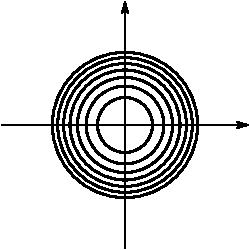
\includegraphics[scale=0.7]{01paraboloidLevels.pdf}
  \quad
  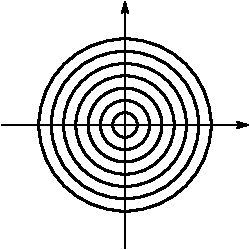
\includegraphics[scale=0.7]{01coneLevels.pdf}
\end{center}
\answer%{{{2
The level sets of the function whose graph is a cone are equally spaced circles
(the level set at level $c$ is a circle with radius $c$).  Hence the one on the
right corresponds to the cone, and
the one on the left corresponds to the paraboloid.
\endanswer


\section*{Problems about movies} %{{{1
\problem  Describe the ``movie'' that goes with each of the following%{{{2
functions.

\subprob $f(x, t) = x\sin t$\hspace{6em}
\answer%{{{2
At time $t$ we have a line through the origin with slope $\sin t$.
As time progresses this lines turns up and down, and up and down,  etc.
\endanswer
\subprob $f(x, t) = x\sin 2t$\hspace{6em}
\answer%{{{2
Same as previous problem, but twice as fast.
\endanswer

\subprob $f(x, t) = t\sin x$
\answer%{{{2
At all times one sees the graph of $y=\sin x$ stretched vertically by a factor $t$.
\endanswer

\subprob $f(x, t) = 2t \sin x$
\answer%{{{2
Same as previous problem, but twice as fast.
\endanswer
\subprob $f(x, t) = t\sin 2x$
\answer%{{{2
The graph of $y=\sin 2x$ stretched vertically by a factor $t$.
\endanswer

\subprob $f(x, t) = (x-t)^2$
\answer%{{{2
Parabola with its minimum on the $x$-axis at $x=t$.
So we see the parabola $y=x^2$ translating from the left to the right
with constant speed 1.
\endanswer

\subprob $f(x, t) = (x-\sin t)^2$
\answer%{{{2
Parabola with its minimum on the $x$-axis at $x=\sin t$.
So we see the parabola $y=x^2$ translating back and forth horizontally
every $2\pi$ time units.
\endanswer

\subprob $f(x, t) = (x-t^2)^2$

\subprob $f(x, t) = \dfrac{t^2}{1+x^2}$

\subprob $f(x, t) = \dfrac{1}{(1+x^2) (1+t^2)}$
\answer%{{{2
At time $t$ we see Agnesi's witch, i.e. the graph $y= a/(1+x^2)$
with amplitude $a=1/(1+t^2)$.  Thus we see a bump whcich starts out small
 at $t=-\infty$, grows to its maximal size at time $t=0$, and then decays
again, until it vanishes at $t=+\infty$.
\endanswer


\problem
\label{prb:01traveling-waves}
If $y=g(x)$ is any function of one variable, then a function of the
form $f(x, t) = g(x-ct)$ is often called a \emph{traveling wave} with
wave speed $c$ and profile $g$.  Let $g$ be any non constant
function of your choice and describe the movie presented by the
function $f(x, t) = g(x-ct)$ (can't choose?  Then try ``Agnesi's
witch'' $g(x) = \frac{1}{1+x^2}$.)

The number $c$ is called the wave speed.  If $c>0$ is the motion to
the left or to the right? Explain.
\answer%{{{2
The graph of $y=g(x-a)$ is obtained from the graph of $y=g(x)$ by
translating the graph of $y=g(x)$ by $a$ units to the right.

Hence the graph of $g(x-ct)$ is the graph of $g(x)$ translated by $ct$
units to the right.  As time changes the graph of $g(x-ct)$ therefore
moves with velocity $c$ to the right.
\endanswer


\problem If $y=g(x)$ is any function of one variable, then a function%{{{2
of the form $f(x, t) = \cos(\omega t) g(x)$ is often called a
\emph{standing wave.}
Let $g$ be any non constant function of your choice and describe the
movie presented by the function $f(x, t) = \cos(\omega t)g(x)$
(can't choose?  Then try ``Agnesi's witch''  $g(x) = \frac{1}{1+x^2}$
again, or for this example, try $g(x) = \sin x$.)

The number $\frac\omega{2\pi}$ is called the frequency of the standing
wave.  The function $g(x)$ is called its profile.  How long does it
take before the standing wave returns to its original position, i.e.\
what is the smallest $T>0$ for which $f(x, T) = f(x, 0)$ for all $x$?
Explain.

\answer%{{{2
If you know the graph of a function $y=g(x)$, then you get
the graph of $y=cg(x)$ by stretching the graph of $g$ vertically by
a factor $c$ (here $c$ is a constant.)
If you allow this constant to depend on time, e.g.\ as in this
problem by setting $c=\cos(\omega t)$, then the ``movie'' you get is of a
version of the graph of $g$ which is growing and shrinking vertically.

\begin{center}
    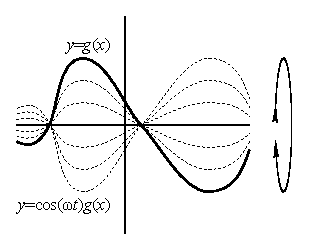
\includegraphics{01standingwave.pdf}
\end{center}
\endanswer


\section*{About open and closed sets} %{{{1

\problem Draw the sets $G_1, G_2, G_3$ from section%{{{2
\ref{sec:openClosedExample} in the same style as
figure~\ref{fig:01openANDclosed} (i.e.\ shade the points in the region
and mark the boundary points which are included in the region).

\problem Using the intuitive description of when a set is open,%{{{2
closed, or neither of those, discuss which of the intervals $(0,1)$,
$[0,1]$, $[0,1)$, and $(0,1]$ are open/closed/neither.

\problem (for discussion) Can you split the plane into two sets, both%{{{2
of which are open?

\rmfamily\normalsize
%\end{multicols}

\section{Continuity and Limits} %{{{1

\subsection{The limit of a function of two variables} %{{{2
Just as with functions of one variable we need to define the limit of
$f(x, y)$ as $(x, y)$ approaches some given point $(a, b)$.
There is again a precise definition involving epsilons and deltas, and
it is in many ways pretty much the same definition as in math 221.
Here it is:
\begin{definition}
  Let $f(x, y)$ be a function of two variables. Then we say that
  $$
  \lim_{(x, y) \to (a, b)} f(x, y) = L
  $$
  if for every $\varepsilon>0$ you can find a $\delta>0$ such that for
  all points $(x, y)$ one has
  \[
  \text{$(x, y)$ lies in $B_{\delta}(a, b)$} \implies
  |f(x, y) - L| <\varepsilon.
  \]
  \label{def:01limit}
\end{definition}

Remember that $B_\delta(a, b)$ is the disc with radius $\delta$ and
center $(a, b)$.  The last line of the definition therefore says that
you can be sure that $f(x, y)$ will be approximately equal to
$L$ with an error of no more than $\varepsilon$, provided you choose
$(x, y)$ so close to $(a,b)$ that the distance between $(x, y)$ and
$(a,b)$ is less than $\delta$.  The first part of the definition will
say that, no matter which $\varepsilon>0$ you come up with, a
$\delta>0$ can be found for which the second part is true.

In this course we will hardly ever use the above definition.  When we
have to compute limits we will use the limit properties, such as
\begin{gather}
  \lim_{(x, y) \to (a, b)} f(x, y) \pm g(x, y) =
  \Bigl\{\lim_{(x, y) \to (a, b)} f(x, y)\Bigr\}
  \pm
  \Bigl\{\lim_{(x, y) \to (a, b)} g(x, y)\Bigr\},
  \\
  \lim_{(x, y) \to (a, b)} f(x, y)g(x, y)
  =
  \Bigl\{\lim_{(x, y) \to (a, b)} f(x, y)\Bigr\}
  \quad\cdot\quad
  \Bigl\{\lim_{(x, y) \to (a, b)} g(x, y) \Bigr\}
  \\
  \lim_{(x, y) \to (a, b)} \frac{f(x, y)}{g(x, y)} =
  \frac{\DS
  \lim_{(x, y) \to (a, b)} f(x, y)}
  {\DS\lim_{(x,y)\to(a,b)} g(x, y)}
\end{gather}
where the latter holds only if $\lim_{(x, y) \to (a, b)} g(x, y) \neq
0$, and the interpretation of these formulas is that \emph{if} the
expression on the right exists, \emph{then} the limit on the left also
exists, and both are equal.

\begin{definition}[Definition of Continuity]
  \label{sec:def-of-continuity}
  A function $f(x, y)$ is called \emph{continuous} at a point
  $(a,b)$ in its domain if
  \[
  \lim_{(x,y) \to (a,b)} f(x, y) = f(a,b).
  \]
\end{definition}

The precise meaning of continuity is expressed in terms of
$\varepsilon$'s and $\delta$'s, using definition \ref{def:01limit},
but the more important interpretation (for this course) of the
definition is that if $f$ is continuous at $(x=a, y=b)$, then the
function value $f(x, y)$ will be close to $f(a, b)$ if $x$ and
$y$ are both sufficiently close to $a$ and $b$, respectively.

In math 234 we do not study the techniques that can be used to prove
continuity of a function of two variables.  While there are many
discontinuous functions, most of these involve division by zero (see
examples below), or ``definition by parts'' (see problem
\ref{prb:stepfunction}), or more complicated constructions.

\begin{figure}[th]\centering
  \framebox{
  \begin{minipage}{0.49\textwidth}\sffamily\null
    \begin{center}
      \bf Iterated Limits
    \end{center}
    Along path 1 you first send $x\to a$, and then $y\to b$, and this
    corresponds to the iterated limit
    \[
    \lim_{y\to b}\lim_{x\to a} f(x, y).
    \]
    If you first let $y\to b$ and then let $x\to a$, you get path 2,
    which corresponds to the other iterated integral.

    There are many other paths along
    which $(x, y)$ can approach $(a,b)$, and the limit
    \[
    \lim_{(x,y)\to (a,b)}f(x, y)
    \]
    equals some number $L$ if $f$ approaches this value no
    matter which path $(x, y)$ follows as it approaches $(a,b)$.
  \end{minipage}
  \begin{minipage}{0.49\textwidth}\sffamily
    \centering

    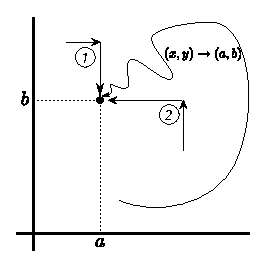
\includegraphics{01limitpaths.pdf}

  \end{minipage}

  }
\end{figure}

\subsection{Iterated limits} Instead of introducing a brand new %{{{2
definition of ``limit'' you could try to recycle the old one-variable
definition of limit.  Thus, in order to find the limit of $f(x, y)$ as
$(x,y)$ approaches some point $(a,b)$, you could first forget about
$y$ and just let $x$ approach $a$.  This leads to
\[
\lim_{x\to a}f(x, y)  = L(y).
\]
This is a limit of one variable, because we're freezing the $y$
variable for the moment.  The result is some quantity which will
depend on the value at which we froze $y$.  Next you could let
$y$ approach $b$, and compute
\[
\lim_{y\to b} L(y) = \lim_{y\to b}\bigl\{\lim_{x\to a}f(x, y)\bigr\}.
\]
The result of this computation would then be our answer to the question
``what happens to $f(x, y)$ when $(x, y)$ goes to $(a, b)$?''

The problem here is that there are at least two versions of this
approach, depending on which limit you take first. You could compute
\[
\lim_{y\to b}\bigl\{\lim_{x\to a}f(x, y)\bigr\}
\text{ and }
\lim_{x\to a}\bigl\{\lim_{y\to b}f(x, y)\bigr\}.
\]
Do these always give the same result?  And do they give the same
result as the limit which we defined above in
\S\ref{sec:def-of-continuity}.  The answer to these questions is
``yes, most of the time, but not always.''

\subsection{Theorem on Switching Limits}\label{sec:01switching-limits} %{{{2
\itshape \textbf{If} $\lim_{(x,y)\to (a, b)} f(x, y) = L$ exists,
\textbf{then} the two iterated limits exist, and they are the same:
\[
\lim_{x\to a}\lim_{y\to b} f(x,y) = \lim_{y\to b}\lim_{x\to a} f(x,y)
= L.
\]
Also, if $\lim_{(x,y)\to (a, b)} f(x, y) = L$ exists, and if $x(t)$
and $y(t)$ are any two functions with
\[
\lim_{t\to t_0} x(t) = a, \text{ and }
\lim_{t\to t_0} y(t) = b,
\]
(so that $(x(t),y(t))$ represents a path which approaches the point
$(a,b)$ as $t\to t_0$) then
\[
\lim_{t\to t_0}f(x(t), y(t)) = L.
\]

\upshape

\subsection{Limit examples} %{{{2
\label{sec:limit-examples}
The function $f(x, y) = (x^2-y^2) / (x^2+y^2)$ is defined everywhere
on the plane, except at the origin.  You could try to assign a value
to $f(0,0)$ by taking the limit of $f(x,y)$ as $x$ and $y$ go to zero.
This is what you find :

Consider the limits
\[
A = \lim_{x\to 0}\lim_{y\to 0} \frac{x^2-y^2}{x^2+y^2} \text{ and }
B = \lim_{y\to 0}\lim_{x\to 0} \frac{x^2-y^2}{x^2+y^2}.
\]
Then you can easily compute that $A=1$ and $B=-1$.  So here is an
example where switching the order of limits changes the outcome.
The theorem tells us that the limit
\[
\lim_{(x, y) \to (0,0)} \frac{x^2-y^2}{x^2+y^2}
\]
does not exist.

Note that to make this example we had to divide by zero at $(0,0)$.

\begin{figure}[ht]\centering
  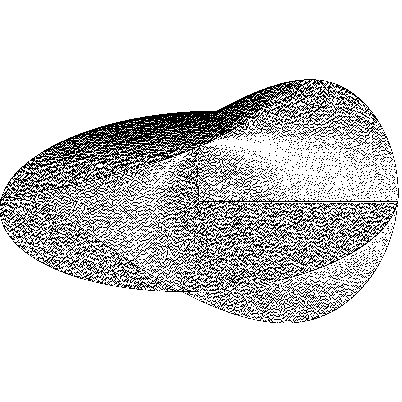
\includegraphics[scale=1.4]{01disco.pdf}
  \caption{The graph of a function which is discontinuous at the
  origin. (See Problem \ref {prb:01disco-axes}.)}
  \label{fig:01disco}
\end{figure}

Here is another example: consider the function
\[
g(x, y) = \frac{2xy}{x^2+y^2}.
\]
Its domain is the whole plane, except the origin, where we once again
would have to divide by zero.

The iterated limits exist for this example.  If you try to compute
them you will find
\[
\lim_{x\to 0}\lim_{y\to 0} \frac{2xy}{x^2+y^2} = 0, \text{ and }
\lim_{y\to 0}\lim_{x\to 0} \frac{2xy}{x^2+y^2} = 0 .
\]
Nevertheless, the limit $\lim_{(x, y) \to (0,0)} g(x, y)$
\emph{does not exist}.  One way to see that is to let $(x, y)$
approach the origin along a straight line, say the line with equation
$y=x$. (What happens along other lines is one of the exercises).
You get
\[
\lim_{x\to 0, \; y=x} g(x, y) =
\lim_{x\to 0} g(x, x) =
\lim_{x\to 0} \frac{2x\cdot x}{x^2+x^2} = 1.
\]
Conclusion: along the $x$-axis and along the $y$-axis $g$ remains 0, but
along the diagonal the function has the value $1$, so that its limit along
the diagonal is 1.



\section{Problems} %{{{1

\begin{multicols}{2}\problemfont

\problem Find the level sets of the functions $f$ and $g$ from%{{{2
\S\ref{sec:limit-examples}.
\answer%{{{2
The level set at level $z=c$ is the set of points which satisfy
the equation
\[
\frac{x^2-y^2} {x^2+y^2} = c.
\]
You can simplify this equation by rewriting it as follows:
\begin{multline*}
  \frac{x^2-y^2} {x^2+y^2} = c \iff\\
  x^2-y^2 = cx^2+cy^2 \iff\\
  (1-c)x^2 = (1+c)y^2 \iff\\
  \frac{y} {x} = \pm\sqrt{\frac{1-c} {1+c}}.
\end{multline*}
So we see that if $\frac{1-c} {1+c}\geq0$ the level set
consists of two \emph{straight lines}, with the indicated slopes.
This happens exactly when $-1<c<1$.

When $c=\pm1$ we get either the equation $x^2=0$ or $y^2=0$, so
that the corresponding level sets consist of either the $y$-axis
or the $x$-axis.
\endanswer


\problem  Compute the limits of the functions $f$ and $g$ from%{{{2
\S\ref{sec:limit-examples} along the lines $y=mx$, where $m$ is a
constant. Does the result depend on $m$?
\answer%{{{2
For $f$ we have
\[
\lim_{x\to0}f(x, mx) = \lim_{x\to 0}\frac{x^2-m^2x^2} {x^2+m^2x^2}
=\frac{1-m^2} {1+m^2}.
\]
In fact this computation shows that $f$ is constant on lines
of the form $y=mx$, which we already found in the previous problem.
\endanswer


\problem
\label{prb:stepfunction}
Consider the function
\[
f(x, y) =
\begin{cases}
  1 & \text{if $y\geq |x|$} \\
  0 & \text{if $y<|x|$}.
\end{cases}
\]
\subprob Draw the graph of $f$.  What is its domain?
\answer%{{{2
The function has been defined for all $(x,y)$, so
its domain is the whole plane.  The graph looks like this, roughly:

\begin{center}
    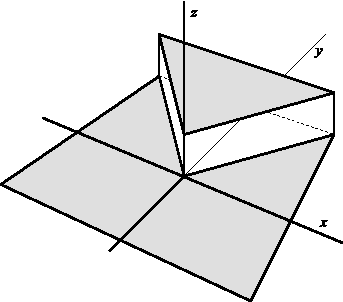
\includegraphics[width=120pt]{01jumpsonabs.pdf}
\end{center}

Note that the drawing doesn't tell you what the function values
are on the jump curve, $y=|x|$.
\endanswer


\subprob Compute the two iterated limits
\[
A=\lim_{x\to0}\lim_{y\to0} f(x, y)
\]
and
\[
B=\lim_{y\to0}\lim_{x\to0} f(x, y).
\]
\answer%{{{2
To compute $A$ we must take the limit as $x\to 0$ of $\lim_{y\to 0}f(x, y)$,
so we must know this limit when $x\neq 0$.

For all $x\neq0$ one has $\lim_{y\to 0}f(x, y) = 0$.
Hence $A = 0$.

To find $B$, compute for any $y\neq 0$
\[
\lim_{x\to0} f(x, y) =
\begin{cases}
  1 & \text{ if }y>0\\
  0 & \text{ if }y<0.
\end{cases}
\]
Hence the iterated limit
\[
\lim_{y\to0}\lim_{x\to0} f(x, y)
\]
does not exist (limits for $y\nearrow 0$ and $y\searrow 0$ are different).

\endanswer


\subprob Compute $\lim_{(x,y)\to(0,0)}f(x,y)$ if it exists.
\answer%{{{2
The limit doesn't exist because one of the iterated limits $A$
and $B$ does not exist.
\endanswer



\subprob At which points $(a,b)$ in the plane is the function
continuous?
\answer%{{{2
The function is continuous at all points $(x,y)$ except those with
$y=|x|$, where the function has a jump discontinuity.
\endanswer


\subprob Answer the same questions for the function
\[
g(x, y) =
\begin{cases}
  1 & \text{if $|x|\leq y\leq 2|x|$} \\
  0 & \text{otherwise}.
\end{cases}
\]

\problem \label{prb:01disco-axes}%{{{2
\subprob Figure \ref{fig:01disco} shows the
graph of
\[
f(x, y) = (x^2-y^2) / (x^2 + y^2)
\]
and the $xy$-plane (the plane $z=0	$).  The axes are missing.
Draw the $x$ and $y$ axes in the figure.

\subprob It turns out that the graph of
\[
g(x, y) = 2xy/(x^2+y^2)
\]
also looks like Figure~\ref{fig:01disco}.  Assuming that
Figure~\ref{fig:01disco} is in fact the graph of $g$, draw the
$x$ and $y$ axes in Figure~\ref{fig:01disco}.

\problem  Let%{{{2
\[
h(x,y) = \frac{x^4-y^2}{x^4+y^2}.
\]

\subprob Compute the limit of $h(x, y)$ as $(x,y)$ approaches the
origin along the line $y=mx$.  Does the result depend on $m$?
\answer%{{{2
\begin{align*}
  \lim_{\substack{(x, y)\to(0,0)\\y=mx}}& h(x,y)\\
  &=\lim_{x\to 0} h(x, mx)\\
  &=\lim_{x\to0} \frac{x^4 - m^2x^2} {x^4+m^2x^2}\\
  &=\lim_{x\to0} \frac{x^2 - m^2} {x^2+m^2}.
\end{align*}
If $m\neq0$ then this limit is
\[
\frac{-m^2} {m^2} = -1
\]
But when $m=0$ you get
\[
\lim_{x\to0} \frac{x^2 - m^2} {x^2+m^2}
=\lim_{x\to0} \frac{x^2} {x^2}
=1.
\]
\endanswer


\subprob Compute the limit of $h(x, y)$ as $(x,y)$ approaches the
origin along the parabola $y=mx^2$.  Does the result depend on $m$?
\answer%{{{2
The two iterated limits
\[
\lim_{x\to0}\lim_{y\to0} h(x, y) = 1
\]
and
\[
\lim_{y\to0}\lim_{x\to0} h(x, y) = -1
\]
are different, so the limit $\lim_{(x,y)\to(0,0)}h(x, y)$ does not exist.
\endanswer


\subprob Does the limit $\lim_{(x,y)\to(0,0)}h(x, y)$ exist?

\subprob Answer the same questions for the function
\[
k(x, y) = \frac{yx^2}{y^2+x^4}.
\]
\answer%{{{2
\begin{align*}
  \lim_{\substack{(x, y)\to(0,0)\\y=mx^2}}& h(x,y)\\
  &=\lim_{x\to 0} h(x, mx^2)\\
  &=\lim_{x\to0} \frac{x^4 - m^2x^4} {x^4+m^2x^4}\\
  &=\lim_{x\to0} \frac{1 - m^2} {1+m^2}\\
  &=\frac{1 - m^2} {1+m^2}.
\end{align*}
So the answer does depend on $m$, i.e.\ depending
on which parabola $y=mx^2$ you follow to get to the origin,
you get a different limit.
\endanswer


\problem The following function plays an important role in the theory%{{{2
of heat conduction, the theory of diffusion, and in probability
theory.  It is called the ``heat kernel'' or ``Gauss kernel''.
\[
H(x, t) = \frac{1}{\sqrt{t}} e^{-{x^2}/{t}}?
\]
Does the limit of $H(x, t)$ at $(0,0)$ exist?  Do any of the iterated
limits exist? More precisely,

\subprob Find $\DS \lim_{x\to 0}\lim_{t\searrow 0} H(x, t)$.

\subprob Find $\DS \lim_{t\searrow 0}\lim_{x\to 0} H(x, t)$.

(The domain of this function is all points $(x,t)$ with $t>0$ -- why?)

A hint:  How do you find the limit $\lim_{s\searrow
0}\frac{1}{\surd s}e^{-1/s}$?  You substitute $s=1/z$, so when $s\searrow 0$
you have $z\to+\infty$, and $\lim_{s\searrow 0}\frac1{\surd s} e^{-1/s} =
\lim_{z\to\infty} \sqrt z e^{-z}$.  Now use your math 221 limits.

\end{multicols}


% vim: tw=80 fdm=marker
